%-*- program: xelatex -*-        
%-*- program: biber -*-`        
%-*- program: xelatex -*-
\documentclass[11pt]{article}
\usepackage[margin=0.75in]{geometry}            % See geometry.pdf to learn the layout options. There are lots.
\geometry{letterpaper}  
\usepackage{amsmath,textcomp,amssymb,geometry,graphicx,enumerate,upquote,color}
\usepackage{hyperref}
\usepackage{breqn}
\usepackage{float}
\usepackage{tikz}
\usepackage{array}
\usepackage{float}
\usepackage{stfloats}
\usepackage{amsfonts}
\usepackage{wrapfig,lipsum,booktabs}
%\usepackage[T1]{fontenc}
%\usepackage[utf8]{inputenc}
%\usepackage{babel}
%\usepackage[font=small,labelfont=bf]{caption}

\def\Session{Fall 2015}
\usepackage[english]{babel}
\title{Risk Measures and Serial Correlation}
\author{Boying Gong, Xinyue Zhou}
\newenvironment{qparts}{\begin{enumerate}[{(}a{)}]}{\end{enumerate}}
\def\endproofmark{$\Box$}
\newenvironment{proof}{\par{\bf Proof}:}{\endproofmark\smallskip}
\begin{document}
\maketitle

% \tableofcontents

% \clearpage

\begin{abstract}
Conditional Expected Drawdown (CED), the tail mean of maximum drawdown distribution, is a newly proposed positive homogenous and convex risk measure. Since maximum drawdown is defined as the accumulative loss from peak to trough, we expect CED to be inherently path dependent and account for serial correlation. Most currently widely-used risk measures such as Value at Risk (VaR), Expected Shortfall (ES) and volatility are based on daily returns and do not account for consecutive losses. We compared CED with these risk measures and show that CED is more sensitive to serial correlation on empirical and theoretical perspective. 
\end{abstract}

\section{Introduction}

Firms and regulators constantly quote risk measures such as VaR, ES and volatility to gauge the amount of asset needed for potential losses. These risk measures are usually calculated from the daily return distribution, thus only accounts for daily losses. However, during the events when consecutive losses happen such as 2008 financial crisis, these measures would become less informative due to the failure to consider the serial correlation of returns. Noticing this drawback of traditional risk measures, Goldberg and Mahmoud\cite{goldberg2014convex} developed Conditional Expected Drawdown (CED), a new risk measure defined over the empirical distribution of maximum drawdown. In this paper, we examine the relationship between serial correlation and various risk measures including CED. 

\subsection{Risk measures}

In the rest of the paper, we mainly focus on the comparison of CED and three extensively studied risk measures including Value at Risk (VaR), Expected Shortfall (ES) and volatility.

\begin{itemize}
\item $\textit{Conditional Expected Drawdown (CED)}$ is defined as the tail mean of maximum drawdown distribution.
\begin{equation}
CED_\alpha(X_{T_n}) = \mathbb{E}(\boldsymbol{\mu}(X_{T_n})|\boldsymbol{\mu}(X_{T_n}) > DT_\alpha).
\end{equation}
where $\alpha$ is the significance level, $DT_\alpha$ is the $\alpha$ quantile of maximum drawdown distribution, $\boldsymbol{\mu}(X_{T_n})$ represents $\textit{Maximum drawdown}$. In the return path of length n, the maximum drawdown is defined by
\begin{equation}
\boldsymbol{\mu}(X_{T_n}) = \mathrm{max_{1 < i < j \leq n} max}({X_{t_i}-X_{t_j}, 0}).
\end{equation}
Maximum drawdown is interpreted as the largest accumulative loss from peak to trough. For the detailed description of CED and its properties including path-dependency, convexity, and positive homogeneity, we direct the interested reader to Goldberg and Mahmoud\cite{goldberg2014convex}.


\item $\textit{Value at Risk (VaR)} $ estimates the potential loss of financial investment in a period. VaR is widely used by investment industry to assess the amount of assets needed to cover possible losses. For a given significant level $\alpha$, VaR is defined as the $\alpha$ quantile of the asset return distribution, which suggests the probability that the amount of loss excess VaR($\alpha$) is less than $\alpha$. The mathematical representation of VaR is: 
\begin{equation}
VaR_{\alpha}(L) = inf\{l \in \mathbb{R} : P(L > l) \leq 1-\alpha \} = 
inf\{l \in \mathbb{R} : F_L(l) \geq \alpha \}.
\end{equation}

\item $\textit{Expected shortfall (ES)}$ is a risk measure which resembles VaR but satisfies monotonicity, translation invariance, homogeneity and subadditivity. The ES of a financial asset is calculated as the tail mean of its return distribution. The Expected shortfall at level $\alpha$ is the expected value of loss which exceeds VaR($\alpha$). It is more sensitive to the shape of the loss distribution especially the tail of the distribution. The mathematical representation of ES is:
\begin{equation}
ES_{\alpha}(L) = E\left[ L \vert L<VaR_{\alpha}(L) \right].
\end{equation}

\item $\textit{Volatility}$ is measured by the standard deviation of asset returns. Higher volatility usually implies greater risk. Under the normality assumption of returns, volatility is proportional to VaR and ES. Although real world asset returns often have fatter tails than normal, volatility is often strongly correlated with VaR and ES, which we will see in later analysis. 

\end{itemize}

\subsection{Serial correlation}

Serial correlation, also known as autocorrelation, is the correlation of observations at different time point. Under the wide-sense stationary process assumption, the serial correlation of $X$ between two time point $t$ and $s$ can be measured by the autocorrelation function as follows:

\begin{equation}
R(\tau) = R(s, t) = \frac{E[(X_t-\mu)(X_s-\mu)]}{\sigma^2}.
\end{equation}

where $\tau = t-s$.

Serial correlation is often associated with the violation of efficiency market and random walk hypothesis. The literature documenting empirical serial correlation is extensive in the late 1980's\footnote{See Barucci and Emilio (2012, Section 6.5) \cite{barucci2012financial} for a detailed review.}. In stock price, Lo and MacKinlay (1988) \cite{lo1988stock} argue that returns based on the horizon longer than one year show a significant mean reversion, while Poterba and Summers (1988) \cite{poterba1988mean} detect a mean aversion for weekly and monthly returns. Lo and Mavkinlay (1988) \cite{lo1988stock}, Conrad et al. (1991) \cite{conrad1991components} model the security returns using a positively autocorrelated common component, an idiosyncratic component and a white-noise component. More extensively, the serial correlation has been documented in literature on nonsynchronous trading, which means assets are not traded simultaneously \cite{lo1990econometric}. Mech and Timothy (1993) \cite{mech1993portfolio} present evidence that the autocorrelation is associated with the delaying in price adjustment caused by transaction costs. In hedge fund returns, Getmansky, Lo and Makarov (2004) argue that serial correlation is an outcome of illiquidity exposure and smoothed returns, market inefficiencies, time-varying expected returns  and leverage and incentive fees with high water marks.

Assuming a moving average representation of reported returns, Getmansky, Lo and Makarov (2004) \cite{getmansky2004econometric} show that Sharp Ratio (SR) tends to be overstated and the market beta understated. Cesare, Stork and Vries (2014) \cite{di2014risk} use the similar structure to demonstrate that the reported value-at-risk (VaR) and expected shortfall (ES) are always smaller than or equal to their actual values. Thus, the risks of assets are easily underestimated using standard risk measures, and the investment decisions may be misleading. Although based on serial correlation and smoothing feature of hedge fund returns, their models are as well applicable to other assets with autocorrelated returns. 

\subsection{Synopsis}

The plan of the paper is as follows. In \emph{Part I: Empirical Analysis}, we present empirical studies analyzing daily returns of various assets. Section 2 provides overall and time-varying risk diagnostics stressing both correlation and the difference between CED and other risk measures. In Section 3, we relate serial correlation with risk measures by fitting time series models, includes AR, MA, ARMA and GARCH. In Section 4, we give an empirical analysis of risk contributions by constructing portfolios of different weights. Next in \emph{Part II: Simulations}, we further illustrate properties of CED by generating returns from time series models. Section 5 contains the comparison of risk measures of various models. And we also give the analysis of the relationship between serial correlation and risk measures based on simulated models. Finally in Section 7, we show that higher serial correlation would result in higher drawdown risk concentrations.

\part{Empirical Analysis}

In this part, we provide the empirical analysis for various asset classes including S\&P 500 Index (SPX), Russell 3000 Index (RAY), etc. Detailed descriptions of their date ranges, components, and summary statistics are given in Appendix \ref{App:AppendixA}.

\section{Risk diagnostics}

\subsection{Overall risk diagnostics}

Table \ref{table:Overall_risk} shows the overall values of four risk measures for various assets over their time range. For each of VaR, ES and CED, we present results of two significance levels 90\% and 95\%. Volatility, ES and VaR are on daily-scale to allow comparison between risk measures in the future. 

\begin{table}[bp]
\centering 
\begin{tabular}{ | r || p{1.5cm} | p{1cm} p{1cm} | p{1cm} p{1cm} | p{1cm} p{1cm} | p{1cm} p{1cm} | } 
 \hline
Measures & Volatility & \multicolumn{2}{c|}{VaR(\%)} & \multicolumn{2}{c|}{ES(\%)} &
 \multicolumn{2}{p{2cm}|}{CED(\%)\quad(3 month)} &\multicolumn{2}{p{2cm}|}{CED(\%)\quad(6 month)} \\ 
Levels & & 0.90 & 0.95 & 0.90 & 0.95 & 0.90 & 0.95 & 0.90 & 0.95 \\
  \hline \hline
AGG & 0.32 & 0.29 & 0.40 & 0.50 & 0.66 & 5.60 &  7.72 & 8.12 & 11.45  \\ 
HYG & 0.84 &  0.62 & 1.03 & 1.41 & 2.03 & 18.41 & 24.07 & 26.43 & 30.77 \\ 
TIP & 0.41 &  0.44 & 0.62 & 0.72 & 0.91 & 7.48 & 9.90 & 11.14 & 12.91 \\ 
BCOM & 0.94 &  1.04 & 1.47 & 1.71 & 2.20 & 18.14 & 22.54 & 26.61 & 33.66 \\ 
MXEA & 0.97 &  1.02 & 1.46 & 1.74 & 2.26 & 20.39 & 23.73 & 27.21 & 31.79 \\ 
MXEF & 1.13 &  1.21 & 1.76 & 2.11 & 2.75 & 26.21 & 30.80 & 36.35 & 43.30 \\ 
RAY & 1.09 &  1.11 & 1.62 & 1.95 & 2.56 & 20.65 & 25.64 & 27.81 & 34.08 \\ 
RMZ & 2.30 &  1.91 & 3.00 & 3.99 & 5.62 & 37.30 & 48.41 & 52.04 & 62.41 \\ 
SPX & 0.97 &  0.99 & 1.43 & 1.71 & 2.23 & 18.35 & 22.67 & 25.18 & 30.65 \\ 
USGG10YR & 1.27 & 1.26 & 1.95 & 2.28 & 2.99 & 23.28 & 28.11 & 32.78 & 39.00 \\
 \hline
\end{tabular}
\caption{Overall risk measures for various assets}
\label{table:Overall_risk}
\end{table}

Note that VaR and ES are calculated based on the empirical distribution of daily returns. Another commonly used method would be based on Gaussian distribution assumption. However, in our case where all asset returns are fat-tailed distributed, applying Gaussian distribution would lead to erroneous results. VaR and ES will be overestimated at a lower confidence level and underestimated at a higher level. This discrepancy phenomenon is rather obvious when the return distribution has an extremely fat tail. We include results assuming Gaussian distribution in Appendix A for comparison.
 
The choice of path length is crucial for CED calculation. As shown in Table \ref{table:Overall_risk}, the value of CED is sensitive to path length. Here we present the CED with rolling three month and six month periods. CED is an increasing function of significance level and path length. We recommend period length no longer than six month for CED estimation. Please refer to an in-depth exploration of behaviour of maximum drawdown distribution and the choice of path length in next subsection. Due to the similarity in definition between CED and ES, they share many features in the calculation. Thus, many ES calculation technique could be implemented for CED estimation. 

While volatility, VaR and ES are strongly correlated with each other across assets, CED has a comparatively weaker correlation with the other three. Note that the four risk measures do not give the same asset sequence from the largest to the least risky asset. Occasionally one risk measure indicates different order under different levels and path length. For example, CED indicates HYG has larger risk than SPX, but other three suggest the opposite comparison result. Moreover, the 6 month CED under 90\% level gives the different relative risk between HYG and BCOM with its counterpart under 95\% level. Notice that the reverse of relative risk suggested by same risk measure for distinct confidence level is more common for CED than for other risk measures.

Back to the economic implications of these risk values. Top three assets in Table \ref{table:Overall_risk} (AGG, HYG, TIP), which are comprised of US bonds, have the smallest risk among all asset class; RMZ, constructed by US equity REITs (Real Estate Investment Trust), have much greater risk than the others; MXEF (MSCI Emerging Market Index), reflecting the emerging market equities, have larger risk than MXEA (MSCI Developed Market Index).

\subsection{Time-varying risk diagnostics}

Time varying risk measures refer to risk measures based on fixed rolling windows. A series of risk measures is obtained. Risk at each time point is given by the past returns of a fixed length. Time-varying risk diagnostics enable us not only to compare risk across assets but to analyze risk for the same asset over time. 

\subsubsection{Maximum dradown distribution}

Unlike VaR and ES, the empirical distribution of maximum drawdown is more sensitive to the time length of measurement. Figure \ref{fig: dmaxdd_RMZ} shows the maximum drawdown of various assets for different path length (3 months, 6 months, 1 year, 2 years, 5 years) separately. As revealed in Figure \ref{fig: dmaxdd_RMZ}, maximum drawdown distribution tends to: a) have the larger mean and variance; b) be multi-mode; c) lack variability of values; d) center around several specific values when we move to longer periods. 

\begin{figure}[bp]
\centering 
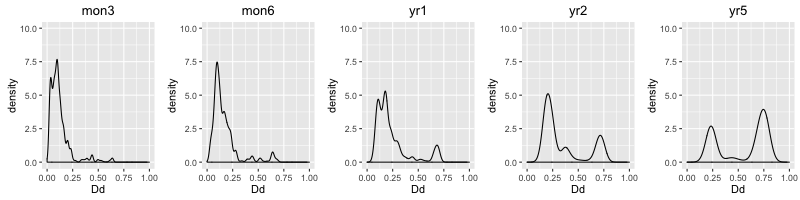
\includegraphics[width = 1\textwidth]{../results/maxdd_RMZ}
\caption{Maximum drawdown distribution of RMZ as rolling period increases} 
\label{fig: dmaxdd_RMZ}
\end{figure}

For daily return data, we do not recommend window length greater than six months for CED estimation. Large drawdowns in real-world asset returns are usually associated with particular events during a short time, for example, the 2008-2009 financial crisis. When considering longer path such as two years or five years, maximum drawdown values tend to be dominant by these events. The empirical distribution would only be defined on several distinct values. In such cases, the empirical quantile no longer exists without distributional or polynomial assumptions of the tail. Thus, it becomes hard to calculate the tail mean (CED). Later in our analysis, we use three or six-month path length. Figure \ref{fig: dist_mdd} shows the empirical distribution of maximum drawdown under the six-month rolling window for various assets.

\subsubsection{Time varying risk measures}

Under Gaussian distribution, VaR, ES, and volatility are linearly dependent. For empirical data where the return distribution has fat tails and distinct kurtosis, they are still strongly correlated. (With average correlation $>$ 95\% for six months rolling window) Figure \ref{fig: risk_meausre_RMZ} shows the VaR, volatility, ES, and maximum drawdown with rolling six-month periods. Four risk measures share a similar pattern of ups and downs, where the risk shot up during the 2008-2009 financial crisis. 

\begin{figure}
\centering 
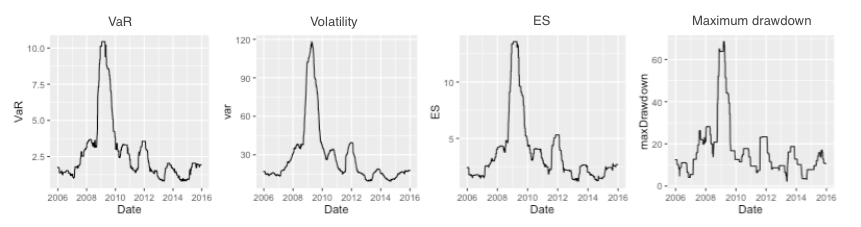
\includegraphics[width = 1\textwidth]{../results/risk_measure_RMZ}
\caption{Comparison of different risk measures of RMZ} 
\label{fig: risk_meausre_RMZ}
\end{figure}

\begin{figure}
\centering 
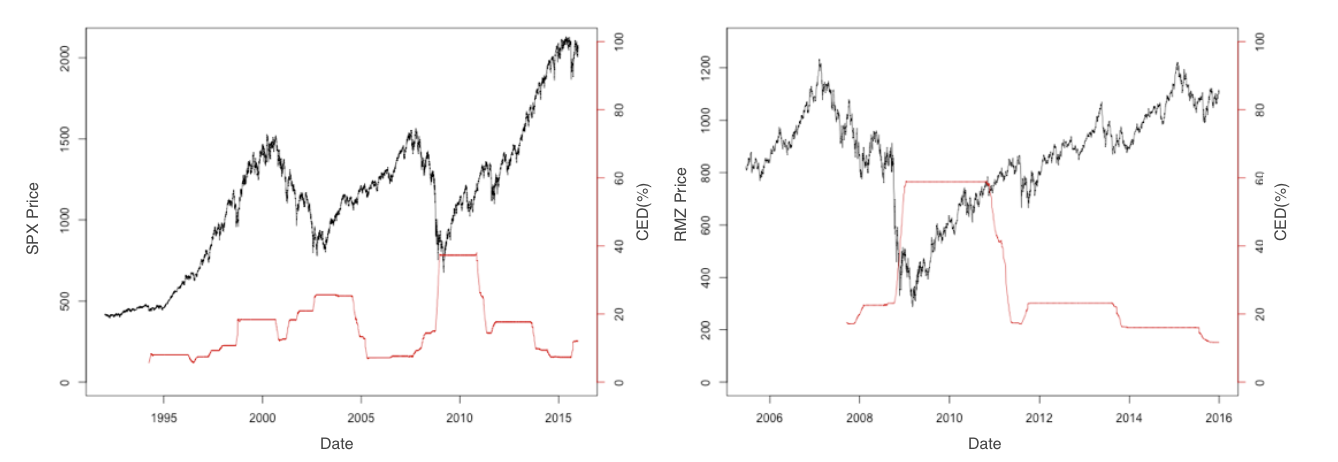
\includegraphics[width = 1\textwidth]{../figures/SPX_RMZ_P_CED}
\caption{Daily price of the S\&P 500 (SPX) and US equity REITs index (RMZ) togther with their 2-year-3month rolling CED.} 
\label{fig:SPX_RMZ_P_CED}
\end{figure}

CED requires more data compared with other risk measures and usually remain constant for a period. To empirically estimate the drawdown distribution, we often rolling a fixed path length. Credible quantile estimation requires hundreds of rollings. For example, two-year-three-month CED evaluates the three-month drawdown risk over the past two years. Figure \ref{fig:SPX_RMZ_P_CED} shows the daily price of the S\&P 500 (SPX) and US equity REITs Index (RMZ) together with their two-year-three-month rolling CED. The CED series also reflect the sharp increase in economic depressions.

CED is closely related to other risk measures. However, the correlation between CED and the other three risk measures are slightly weaker than the correlation among volatility, VaR, and ES. Table \ref{table:corrRiskMeasureCED} shows the correlation between CED and other risk measures calculated based on six-month rolling risk measures for every asset. 

\section{Time series analysis}
%%% add here %%
%%% The reason for time series analysis %%%
\subsection{ARMA} \label{arma}
ARMA is the simplest and most commonly used time series model, which is enable to capture the correlation between current time point and one or several lags in a stationary time series. Therefore, in the section \ref{arma}, ten kinds of U.S indices are feeded into ARMA models, first simple chosen models from the family, then best model through selection steps. From there, one can take the first sight of the relationship between serial correlation and different risk measurements in real-world data.

\subsubsection{Result of basic ARMA model fit}
Started from the simplest ones, ten U.S indices have been feeded into 3 most basic ARMA models: AR(1), MA(1) and ARMA(1,1). The three models here are not necessary the best one, or even the ones that all underlying assumptions are satisfied. This step is just try to have a general idea if the serial correlation of each model is related with risk measurements in some way. When it comes to serial correlation here, it refers to the first order autocorrelation of the time series models. 

Following is a short summary on these three ARMA model, including their formulus, description and the method for calculating the serial correlation.

\begin{enumerate}
\item \textbf{AR(1)}
\begin{itemize}
\item Model:
\begin{equation}
X_t = \phi X_{t-1} + \epsilon_t \ \ \  s.t.\ |\phi | < 1
\end{equation}
\item AR(1) just has the AR component with lag 1 in the ARMA model, which characterized by only the previous term in the process and the noise term contributing to the output. When $\phi$ is closer to 0, the whole process is more like to be white noise.
\item The equation for calculating the serial correlation:
\begin{equation}
\rho(h) = \phi ^h, \ h = 0,1,\dots
\end{equation}
\end{itemize}

\item \textbf{MA(1)}
\begin{itemize}
\item Model:
\begin{equation}
X_t = \epsilon_t + \theta\epsilon_{t-1}
\end{equation}
\item MA(1) just has the MA component with lag 1 in the ARMA model, which impost the shock for the current period and q periods into the future; in contrast, in the AR model a shock affects  X values infinitely far into the future.
\item The equation for calculating the serial correlation:
\begin{equation}
\rho(h) = \begin{cases} \frac{\theta}{(1+\theta^2)} &\mbox{if } h = 1 \\ 
0 & \mbox{otherwise } \end{cases}
\end{equation}
\end{itemize}

\item \textbf{ARMA(1,1)}
\begin{itemize}
\item Model:
\begin{equation}
X_t = \phi X_{t-1} + \epsilon_t + \theta\epsilon_{t-1}
\end{equation}
\item ARMA(1,1) has both AR and MA component with lag 1. ARMA(1,1) is the combination of AR(1) and MA(1), which ACF incorporate the characteristics from both AR and MA: both error term and data point are directely affected by that on the previous time points.
\item The equation for calculating the serial correlation:
\begin{equation}
\rho(h) = \frac{(1+\theta \phi)(\theta + \phi)}{1+ 2\theta \phi +\phi^2} \phi^{h-1}, \mbox{if } h \geq 1
\end{equation}
\end{itemize}
\end{enumerate}
The Table\ref{table:corSerialRisk} shows the correlatio between serial correlation and different risk measures for AR(1) and ARMA(1,1). Figure\ref{fig:SerCol-CED5yr3monAR1} and Figure \ref{fig:SerCol-VaR5yrAR1}
 in the appendix shows a more straightforward relationship between first order serial correlation of AR(1) and risk measures. Consistent with what was showing in the plot, all the assets except MXEA and MXEF have the high correlation between $\kappa(1)$ and risk measurements. Within each asset, as expected, the correlation with VaR and ES are very closed, as VaR is highly correlated with ES internally. However, compared with VaR and ES, the correlation with CED is relatively smaller, and sometimes the correlations are even with different sign.

%\begin{wraptable}{l}{10.5cm}
\begin{table}[H]
\centering 
\begin{tabular}{ | c || r r r|| r r r | } 
 \hline
 &\multicolumn{3}{c|}{AR(1)} &\multicolumn{3}{c|}{MA(1)} \\
 \cline{2-7}
Asset & VaR  & ES & CED & VaR  & ES & CED \\
  \hline \hline
AGG & 0.92 & 0.95 & 0.94  & 0.94 & 0.96 & 0.94  \\ 
HYG & -0.61 & -0.56 &  -0.41 & -0.51 & -0.45 &  -0.29  \\ 
TIP & -0.67 & -0.75 &  -0.73 & -0.65 & -0.74 &  -0.73\\ 
BCOM & 0.86 & 0.80 & 0.76 & 0.86 & 0.80 & 0.76\\ 
MXEA & 0.26 & 0.33 & 0.08& 0.01 & 0.11 & 0.15 \\ 
MXEF & 0.23 & 0.22 & -0.05& 0.15 & 0.16 & -0.12  \\ 
RAY & 0.79 & 0.76 & 0.49 & 0.79 & 0.77 & 0.50 \\ 
RMZ & 0.90 & 0.93 &  0.81 & 0.92 & 0.95 &  0.84\\ 
SPX & 0.62 & 0.70 & 0.15 & 0.65 & 0.72 & 0.17\\ 
USGG10YR & 0.67 & 0.64 &  0.66 & 0.65 & 0.64 &  0.68\\
 \hline
\end{tabular}
\caption{Correlation between $\rho(1)$ and risk measures. The time window used for get risk measurements and $\rho(1)$ is 5 years, and the rolling window within 5 year for CED is 3 month.}
\label{table:corSerialRisk}
\end{table}

Both the table and figures are unable to tell the story what are the relationships between risk measures and serial correlation for the indices, since the model here are recklessly chosen and more complicated factors shocking the market everyday. However, the table provides an idea that relationship with CED is more closed to that with VaR and ES when this correlation is internally large.
%\end{wraptable}

\subsubsection{Model selection}
The model selection is accomplished by trying to find a proper time series model on the unit of all data for each asset, for the fact that it makes no sense to fit different model for each rolling time period within one financial asset.  Unfortunately, observing from the ACF plot of returns, most of them are not stationary by nature without drift term, which means ARMA model is inherently not or just a partial a good selection for fitting them. It may also explain the reason why the previous section did not produce a expected result that CED is more correlated with serial correlation $\kappa(1)$.
\begin{wraptable}{r}{6.5cm}
%\begin{table}[!h]
\caption{Best ARIMA Model for the U.S. Assets }
\centering 
\begin{tabular}{ | c || r | } 
 \hline
Asset & ARIMA (p,d,q) \\
  \hline \hline
AGG & (5,0,5) \\ 
HYG & (3,0,1) \\ 
TIP &  (0,0,0)\\ 
BCOM & (0,0,0)\\ 
MXEA & (2,0,2) \\ 
MXEF & (4,0,2)\\ 
RAY &  (2,0,2)\\ 
RMZ & (0,0,1) \\ 
SPX & (2,0,2) \\ 
USGG10YR & (0,0,0) \\
 \hline
\end{tabular}
\label{table:BestArima}
%\end{table}
\end{wraptable}


Our criterion here for ``better model'' is the smaller AIC value. Appendix \ref{App:AppendixD} provides a more detailed explanation on model select criteria. To confirm the fact that ARMA is not reasonable for almost all the indices, we tried sets of parameter for ARMA and select the one with the smallest AIC value. Essentially, we chose the combination of AR and MA parameters ranging from 1 to 5.  Table \ref{table:BestArima} shows the best selection based on AIC criteria. The Table \ref{table:BestArima} indicates that the parameters are as high as 4 or 5 for almost all the assets, which suggests that the time series are not stationary. It also involved some converging issue is when the parameters are getting too larger.


To illustrate this point, the following is an example analysis on RMZ index. There are several reasons why RMZ is selected: 1) the RMZ has a shorter period, which means it includes less abnormal market shock such as financial crisis in 2008 and more close to the normal fluctuation in stock price. 2) Larger serial correlation and ES, VaR comparing with other indices, implying it is more suitable for analysing the relationship between serial correlation and various risk measures. 3) There are less modes in Maximum drawdown of RMZ, suggesting it is reasonable to get tail mean, which is CED.
\subsubsection{RMZ: an example}
Grid searching of the best parameter set of ARIMA model is applied to RMZ index. On the basis of both AIC and BIC selection criteria (Appendix \ref{App:AppendixD}), MA(1) turns out to be the best option.

\begin{figure}[H]
  \centering
  \begin{minipage}[b]{0.48\textwidth}
  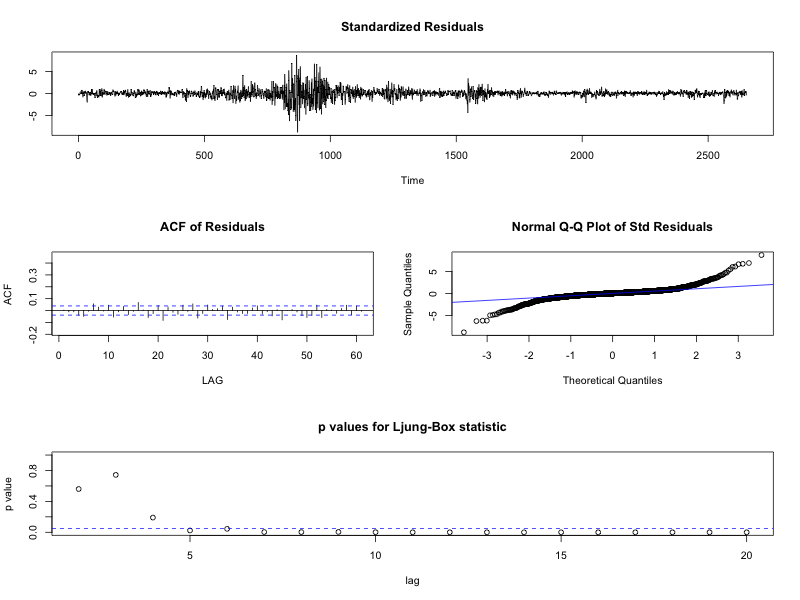
\includegraphics[width = 1\textwidth]{../results/DiagnosticRMZ}
      \caption{Diagnostic Plots of MA(1) for RMZ}
  \label{fig:DiagnosticRMZ}
  \end{minipage}
  \hfill
  \begin{minipage}[b]{0.48\textwidth}
  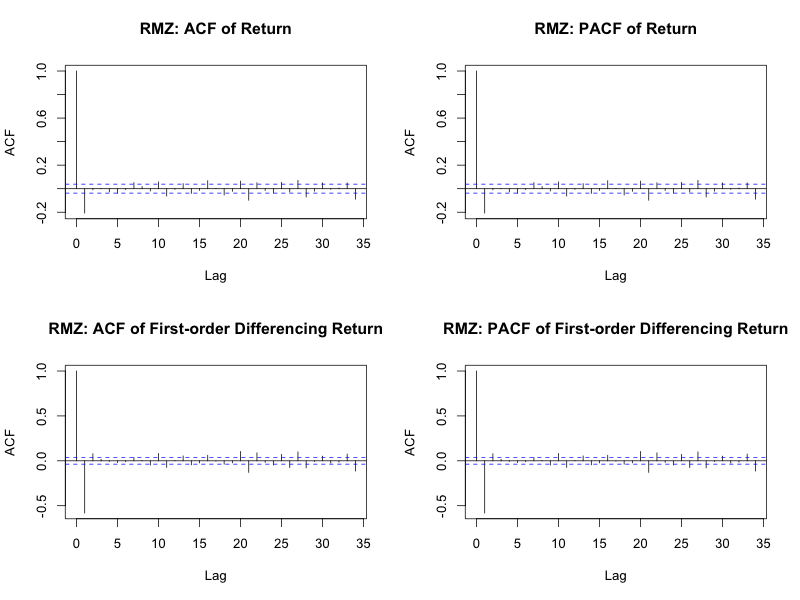
\includegraphics[width = 1\textwidth]{../results/ACFofRMZ}
  \caption{ACF/PACF of Return for RMZ}
  \label{fig:ACFofRMZ}
  \end{minipage}
\end{figure}
However, the residuals after fitting does not convert into white noise as the assumption of ARIMA model. The factors lead this result is complicated and beyond our discussion, as this is a 10-year-long time series and market shock varied during this long time. Figure \ref{fig:DiagnosticRMZ} shows the diagnostic results after the fitting. The variance of residuals are clustered across the time. After taking a closed look at the data, agreed with expectation, the high volatility period is corresponding to 2008 financial crisis.

Figure \ref{fig:ACFofRMZ} also demonstrates this problem in ACF/PACF plot, in which some correlations exist between residuals after more than 50 lags, but they are comparatively small after the fitting.Normal Q-Q shows that residuals are heavy-tailed. Ljung–Box–Pierce Q-statistic, used for test grouped $\kappa_e(h)$, rejects $H_0$ after $5^{th}$ lag, which also indicates the residual is not white noise after fitting. The diagnostics suggest that AR(1), MA(1) and ARMA(1,1) could all be good options, while the time series is not stationary by nature. Therefore, more complicated model should be adopt to capture the pattern with in the variance of residual.



\subsection{GARCH} \label{garch}
For financial assets, the returns have strong dependency across the time, thus it is reasonable to fit time series to interpret and predict them. As described in Section \ref{arma}, the ARIMA models are infeasible for most assets from diagnostics plots, in which the variance cluster in the return could not be captured, resulting in some variance cluster left the residual plot. To solve the problems listed above, the GARCH then is attempted to fit the returns for various assets. It turns out to have a much better performance in capturing the variance, and hence, a reasonable diagnostic plots.
\subsubsection{Why GARCH is better?}
The GARCH is the most widely used the model in financial data fitting. Rather than ARIMA having constant variance assumption, GARCH also model the heteroscedasiticity in the time series.  For GARCH(1,1), the model is discribed as following:
\begin{align*} 
y_t & = \sigma_t \epsilon_t\\
\sigma_t^2 & = \alpha_0+ \alpha_1 y_{t-1}^2 +\beta_1\sigma_{t-1}^2
\end{align*}
These set of formulus in indicates that the current variance of the noise is affected by variance of error in the previous several periods and the magnitude of the previous return. In this model, the clustered variance of residuals can be efficiently captured. Additionally, GARCH also inherits good properties of the ARMA in characterizing the correlation within consecutive time points. Considering all the benefits listed above, GARCH is an ideal model for improving the ARMA mentioned in Section \ref{arma}.

\subsubsection{Result of GARCH fit}
Seen from the returns plot for different assets, the clustered variance is a common case in financial assets. Especially for really long time series, such as \textit{MXEA}, the market shock is even harder to interpret and predict. Therefore, for those assets with long time series, a longer lag of ARMA model is required. The best fit of GARCH model on all the selected assets are shown in the Table \ref{table:BestGarch}.
%\begin{figure}[H]
%  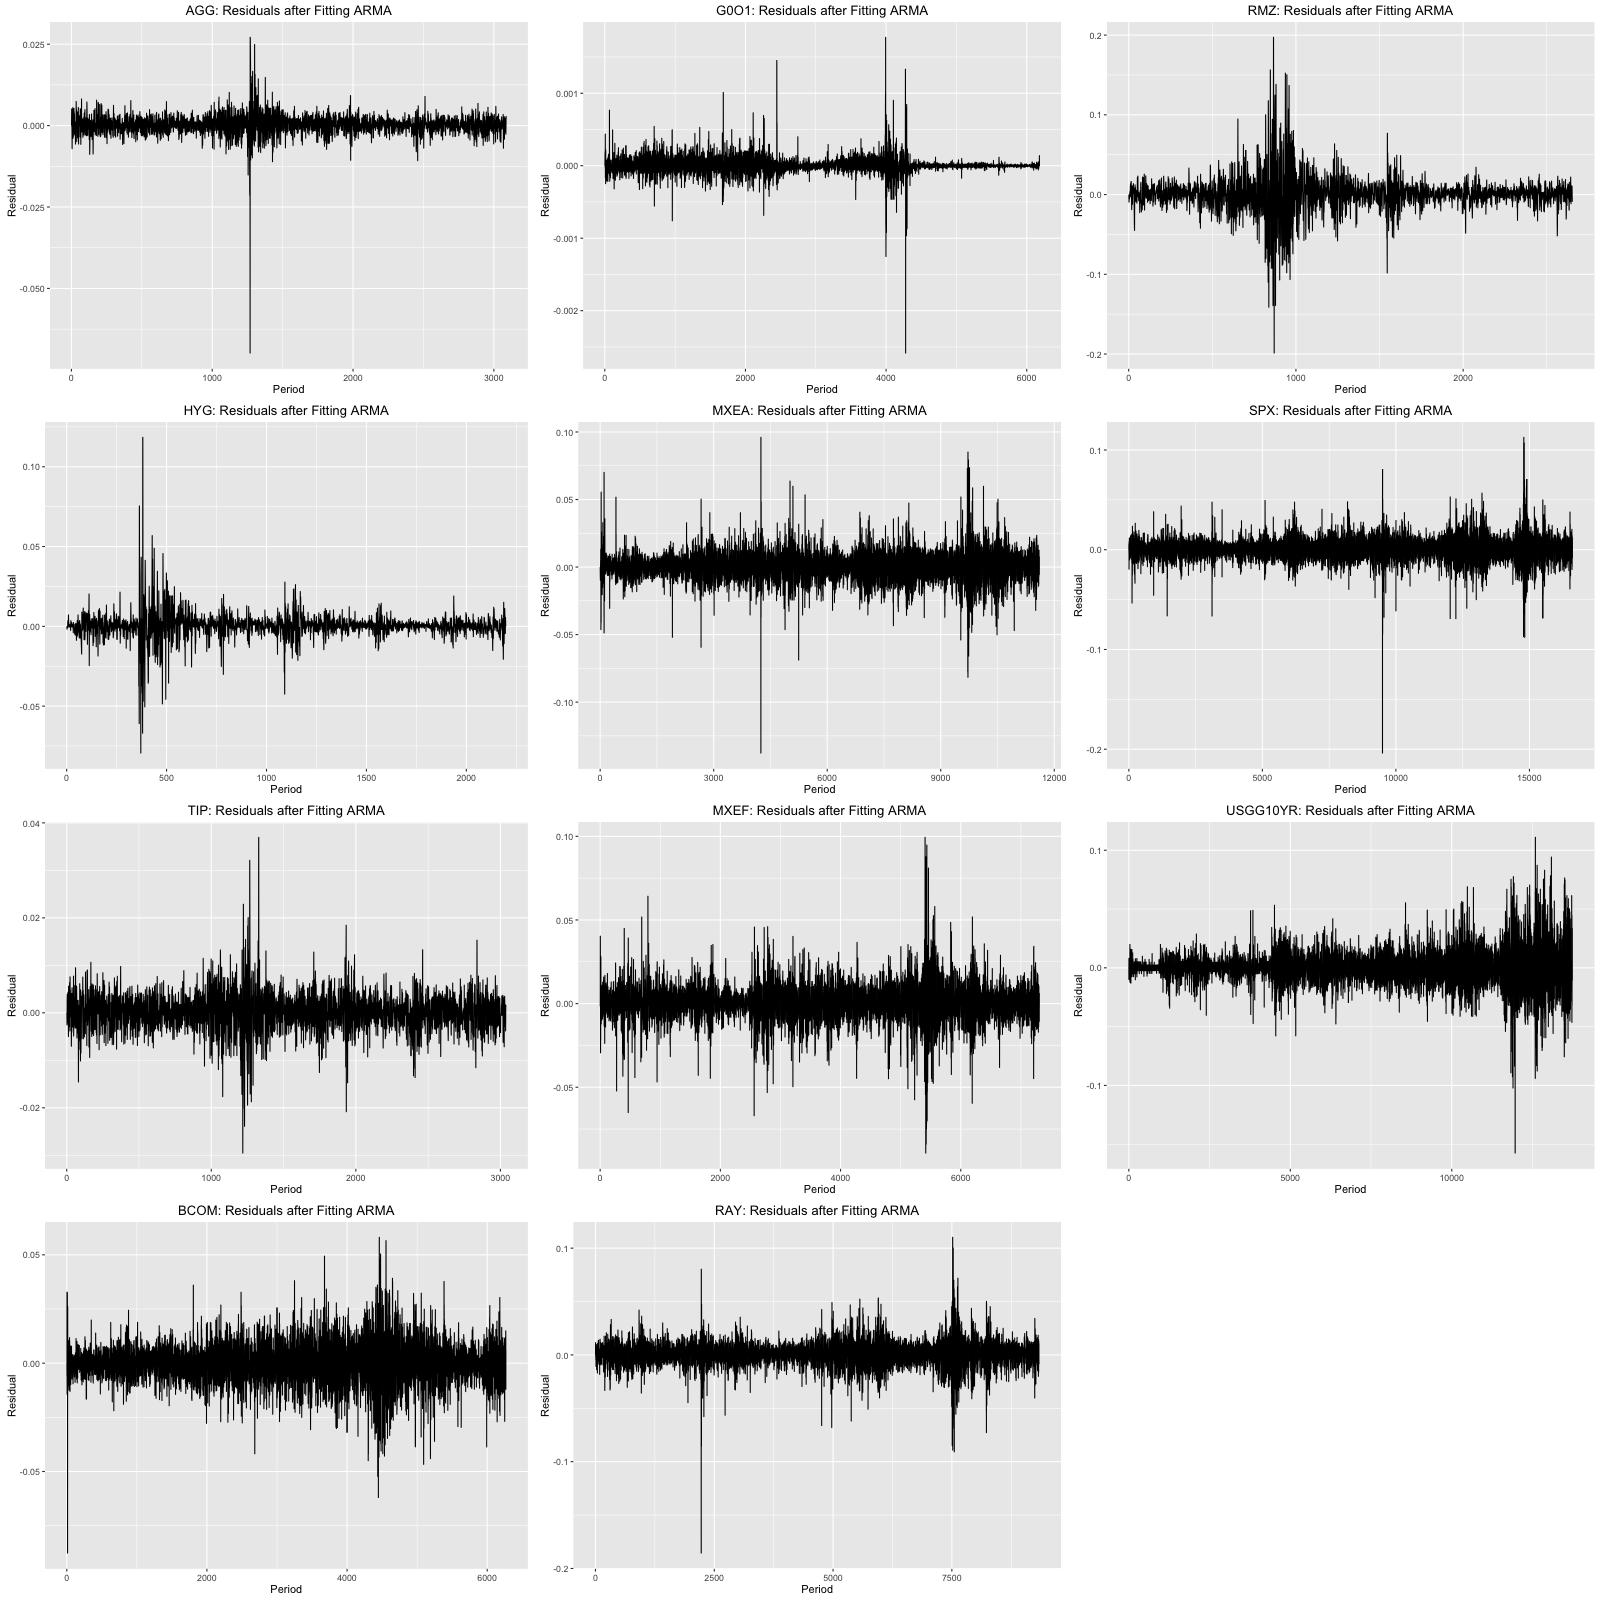
\includegraphics[width = \textwidth]{../results/resids}
 %  \caption{Residuals after fitting using the best ARIMA Model}
%  \label{fig:DiagnosticResids}
%\end{figure}
\begin{table}[!h]
\caption{Best GARCH Model for the residuals after Fitting ARIMA}
\centering 
\begin{tabular}{ | c || c | c | c|} 
 \hline
Asset & ARIMA (p,q)+ GARCH(m,n) & BIC & $\kappa(1)$\\
  \hline \hline
AGG & ARMA(5,5)+GARCH(1,1) & -6.8688 & -0.0698\\ 
HYG & ARMA(3,1)+GARCH(1,1) & -6.8628 & -0.5756\\ 
TIP &  GARCH(1,1)&-8.3838 & 0\\ 
BCOM & GARCH(1,1)&-6.7632 &0\\ 
MXEA & ARMA(2,2)+ GARCH(1,2) &-6.7857 & -0.2176\\ 
MXEF & ARMA(4,2) + GARCH(1,1)&-6.5399 & -0.6328\\ 
RAY &  ARMA(2,2) + GARCH(1,1)&-6.6313 & 0.2526\\ 
RMZ & MA(1) + GARCH(1,1)&-5.6962 & 0 \\ 
SPX & ARMA(2,2) +GARCH(1,1)&-6.8697& 0.3488\\ 
USGG10YR & GARCH(1,3) &-6.664873& 0\\
 \hline
\end{tabular}
\label{table:BestGarch}
\end{table}
The parameters are selected using in-sample error measure BIC. Details about BIC can be found in Appendix \ref{App:AppendixD}. The mean difference between BIC and AIC is that BIC tends to penalty more on complexity and resulting less feature in the model. As garch models are very likely to be overfitting, choosing BIC is of greater reasonability.

The GARCH model highly reduces the correlation within the residual and ends up with a more reasonable dignostics, while the predictivity of the model has  been highly improved( 
%%\ref {}%%!!!!!!!!!!!!!!!!!!!!!!!!!!!
is a good example). However, there are still problems presenting in GARCH model, and needs further solutions to handle it. The heavy tail is existing as the sign from the normal Q-Q plots, in which points deviate from line at both ends. Heavy tail problem is caused by assumption of the Gaussian conditional distribution in GARCH. Instead of Gaussian, t-Student could be used as the conditional distribution is able to catch the variance on both tails. Causing convergency issue time to time by t-Student distribution, Generalize Normal Distribution (GED) and  QMLE are other potential options.
 
\subsubsection{RMZ: an example}
This section presents a model selection and assessment process of the RMZ example on GARCH method, showing a diagnostics of the model and the predictive capability of the model.
%%Section\ref%% 
is highly related to this section, in which GARCH time series are simulated and fitted so that a more clear pattern is generated eliminating all the other market factors. There, we can see a more clear relationship between serial correlation and different risk measures.

First of all, The MA(1)~ GARCH(1,1) for RMZ is estimated as followed:
\begin{align*}
R_t &= -4.1561\times 10^{-2}\epsilon_{t-1} \\
\sigma_t^2 & = 1.9955 \times 10^{-6} +1.1083\times 10^{-1} T_{t-1}^2 +8.8506\times 10^{-1}  \sigma_{t-1}^2
\end{align*}

\begin{figure}[H]
  \centering
  \begin{minipage}[b]{0.48\textwidth}
  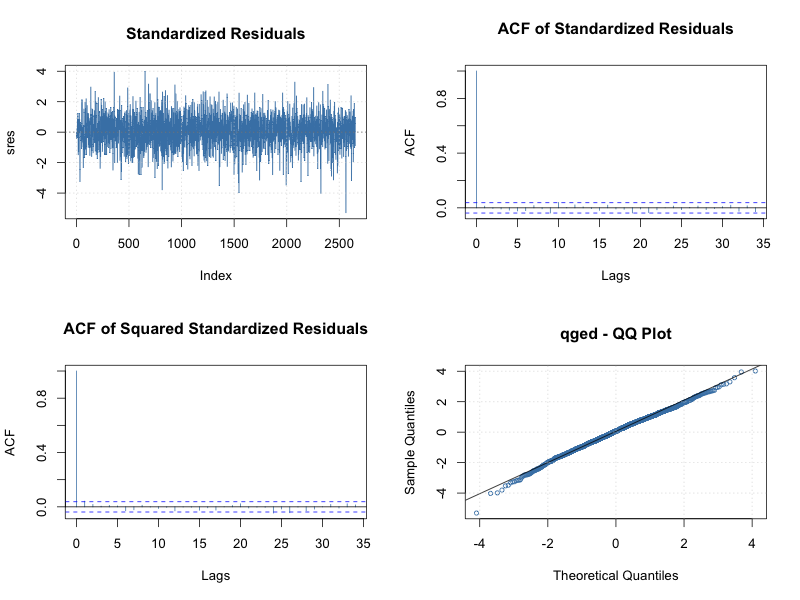
\includegraphics[width = \textwidth]{../results/RMZ_GARCH_dig2}
  \caption{RMZ: Diagnostic Plots of GARCH(1,1) with GED Conditonal Distribution}
  \label{fig:RMZ_GARCH_dig2}
  \end{minipage}
  \hfill
  \begin{minipage}[b]{0.48\textwidth}
   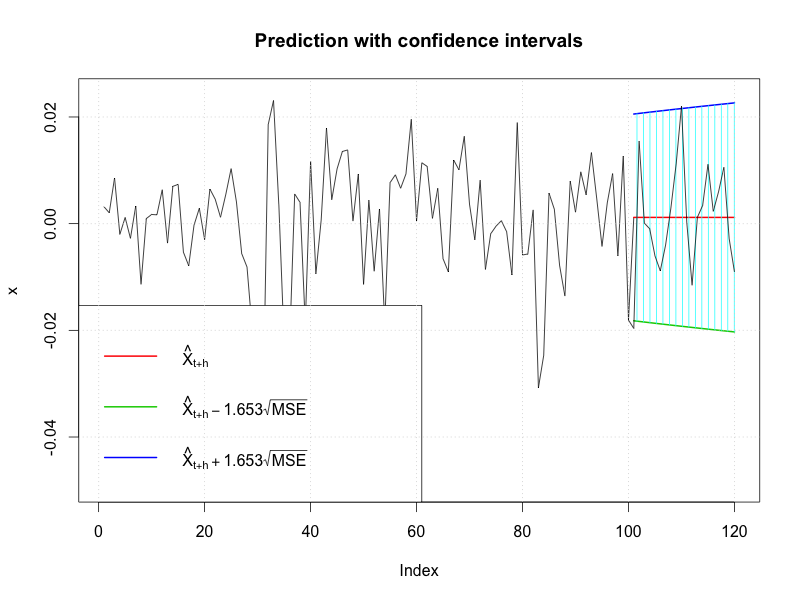
\includegraphics[width = \textwidth]{../results/RMZ_GARCH_predCI}
  \caption{RMZ: Estimate of the Instantaneous Conditional Standard Deviation}
  \label{fig:RMZ_GARCH_predCI}
  \end{minipage}
\end{figure}

Figure \ref{fig:RMZ_GARCH_dig2} shows the diagnostic after fitting GARCH(1,1) with a generialized normal distribution on the residuals of RMZ after the ARMA fitting. The resulting errors feasibly tend to be white noise, without any apparent correlation within them. After apply the heavy tail fixer on conditional distribution using GED, the resulting error is more Gaussian distribution,, following almost exactly to the line in Q-Q plot.

Figure \ref{fig:RMZ_GARCH_predCI} indicates the capability of GARCH in one and several steps prediction. It shows the last 120 residuals from RMZ index, and all but last 20 are used to fit the GARCH(1,1) model with GED conditional distribution.  An confident interval is also created based on mean and standard deviation. And it is nice to see that almost all the last 20 points lies in the interval.

\subsection{Regime dependent analysis}

Most economic time series data behave differently in the adjacent period. For example, asset returns
usually show considerable volatility during a financial crisis. One standard approach to model abrupt changes in regime is to use the Hamilton's Markov regime switching model\cite{hamilton1994time}\cite{hamilton1990analysis}. In our study, we use the following two-regime switching model to fit the returns:

\begin{equation}
y_t - \mu_{s^*_t} = \phi_{s^*_t} (y_{t-1} - \mu_{s^*_{t-1}}) + \epsilon_t
\end{equation}
where the number of autoregressive coefficients is set to 1. $s^*_t$ is a two-state Markov chain. $s^*_t = 1$ represent regime 1 and $s^*_t = 2$ represent regime 2. $s^*_t$ depends on the past only through the most recent values:

\begin{equation}
P(s_t = j|s_{t-1}, s_{t-2}, \dots) = P(s_t = j|s_{t-1})  = p_{ij}
\end{equation}

\subsubsection{Comparison of basic summary of two regimes}

\begin{wraptable}{r}{8.5cm}
% \begin{table}[H]
\centering 
\begin{tabular}{ | c || r r | r r | } 
    \hline
    & \multicolumn{2}{c|}{Regime 1}  & 
    \multicolumn{2}{c|}{Regime 2} \\
     & \multicolumn{2}{c|}{High volatility}  & 
    \multicolumn{2}{c|}{Low volatility} \\
    & $\phi$ & Std & $\phi$ &  Std \\
     \hline \hline
    AGG  & -0.134 & 0.009 & -0.114 & 0.002 \\ 
    HYG & -0.010 & 0.016 & 0.025 & 0.004 \\ 
    TIP &  0.039 & 0.007 & -0.026 & 0.003 \\ 
    BCOM & -0.046 & 0.013 & 0.050 & 0.006 \\ 
    MXEA & 0.095 & 0.015 & 0.109 & 0.006 \\ 
    MXEF & 0.221 & 0.018 & 0.254 & 0.007\\ 
    RAY& -0.039  & 0.019 & 0.052 & 0.007\\ 
    RMZ & -0.244 & 0.040 & 0.007 & 0.010\\ 
    SPX & -0.018 & 0.016 & 0.113 & 0.006\\ 
    USGG10YR & -0.031 & 0.020 & 0.082 & 0.006\\ 
    \hline
\end{tabular}
\caption{Coefficient estimation of two regimes} 
\label{table:autoCoeffRegime}
% \end{table}
\end{wraptable} 

Table \ref{table:autoCoeffRegime} shows the estimated autoregression coefficient $\phi$ and standard deviation of the noise term of two regimes for various assets. We also provide the standard deviation, skewness, and kurtosis of different assets in Table \ref{table:statSumRegime} in the appendix. Note that regime 1 represents high volatility regime while regime 2 represents low volatility one. In general, it is clear that returns of regime 1 have a larger standard deviation, skewness, and kurtosis than that of regime 2. This difference in kurtosis indicates that the return distribution in low volatility regimes has a lighter tail. In contrast, in high volatility regimes, there are more extreme values of returns.

We observe that low volatility regimes are more likely (9 out of 10 assets) to show larger autocorrelation coefficient. Although we expect greater drawdown risk when serial correlation increase (which means more significant autocorrelation coefficients estimate here), we did not prove this through empirical results. Later we will show in the simulation study that given different serial correlation and error term variance of the time series model, the latter factor dominant the impact to CED values, which is the case in our empirical findings. But under the same level of noise term variance, the larger the serial correlation, the greater the CED.

\begin{figure}[H]
    \centering
    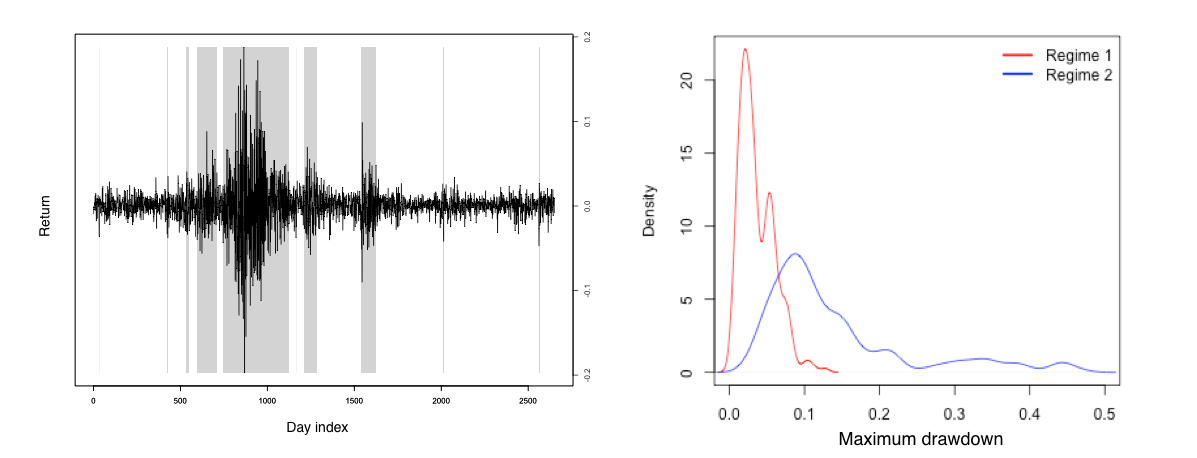
\includegraphics[width=1\textwidth]{../results/regime/RMZ_regime}
    \caption{Left panel: Return plot of RMZ from June 20th, 2005 to December 31st, 2015. Shadowed areas represent regime 1 with high volatility, and white areas indicate regime 2 with low volatility. Right panel: one-month maximum drawdown distribution of regime 1 and regime 2 of RMZ.}
    \label{fig: RMZregime}
\end{figure}

\begin{table}[H]
    \centering 
    \begin{tabular}{| r | r | r |} 
        \hline
        & Regime 1 & Regime 2 \\
        & High volatility & Low volatility \\
        \hline 
        VaR (empirical, p = 0.95) & 7.4\% & 1.5\% \\
        ES (empirical, p = 0.95) & 9.9\% & 2.1\% \\
        CED (one-month, p = 0.9) & 38.4\% & 8.4\% \\
        Serial correlation (order = 1) & -0.257 & -0.026 \\
        Serial correlation (order = 2) & -0.023 & 0.008 \\
        \hline
    \end{tabular}
    \caption{Risk diagnostics for RMZ of two equal-length episode of each regime} 
    \label{table:ridkDiagsRegimeRMZ}
\end{table}

\subsubsection{RMZ: An example}

In order to make a consistent comparison of risk diagnostics between two regimes, we ignore some short discontinuity and pick two longest single occurring episode for each regime. Here we use RMZ, the most risky asset in our data set as an example. Both episode contain 530 trading days. The episode of regime 1 range from October 30th, 2007 to December 7th, 2009, and the episode of regime 2 range from June 20th, 2013 to July 29th, 2015. 

In Figure \ref{fig: RMZregime}, the left panel shows the return of RMZ from June 20th, 2005 to December 31st, 2015. The shadowed area represents the regime with high volatility and the white area low volatility. This model is consistent with the actual financial event in that the high volatility regime covered mainly from mid-2007 to 2010. As we might expect, regime with high volatility also shows high risks in that they have larger ES and VaR values. Moreover, model of regime 1 only explains 26.3\% of the observations, which means abrupt deviation is a minority in total observations. By looking at assets with longer period, we find a similar proportion of high volatility regimes (SPX: 23.7\%, RAY: 20.6\%). The right panel shows the one-month maximum drawdown distribution calculated based on the continuous episode we selected. The maximum drawdown distribution in regime 1 has larger mean and variance as well as greater knewness and kurtosis. 

We may wrongly interpretate that larger serial correlation results in less drawdown risk. Notice from the results in later simulation section that variance of noice term dominant the influence for CED. And we can only obverve the positive correlation between serial correlation and CED under fixed variance level.


\subsection{Other return frequencies}

\section{Empirical risk contribution}
\subsection{SPX \& RMZ: An example}

\part{Simulations}

In this part, we explore the relationship between serial correlation and risk measures by analyzing models from data generated by known time series. Real world financial data is usually more complicated and simultaneously influenced by multiple effects. Simulation allow us to examine one specific factor by fixing others. For example, we may change one coefficient of a time series model while keeping other at the same level, which enables us to examine the relationship of certain order of serial correlation and CED.

\section{Serial correlation and risk measures}

In this section, we simulate various time series models and examine the impact of serial correlation on risk measures.

\subsection{ARMA model}

We started from the simplest model AR(1):

\begin{equation}
X_t = \kappa_1X_{t-1} + \epsilon_t
\end{equation}

We simulate AR(1) for various values of the autoregressive parameter for $\kappa_1 \in (-1, 1)$ . Figure \ref{fig:AR1_risk_measures} shows the relationship between AR(1) coefficient and risk measures of interest including ES, VaR, volatility and CED. Note that for AR(1) model, the order one serial correlation is the the value of autoregressive parameter.

CED shows a decreasing trend when $\kappa_1\in(-1, -0.75)$ and an increasing trend when $\kappa_1 \in(-0.75, 1)$. As shown in Figure \ref{fig:AR1_risk_measures}, it becomes feasible for us to distinguish negative and positive serial correlation using the CED values. However, the other 3 risk measures are all symmetric about $\kappa_1 = 0$, and they increase as the absolute values of $\kappa_1$ increases.

For VaR, ES and CED, the derivative of risk measure values to $\kappa_1$ approaches to zero as  $\kappa_1$ goes to 0 and increase as $\kappa_1$ increase. This suggests that the value of this three risk measures can hardly reflect the change of serial correlation when the serial correlation is small. And they perform better when the serial correlation increases. The trend of derivatives reverse for CED. While the change of $\kappa_1$ has a comparatively larger influence around 0, the influence becomes weaker as we move to larger  $\kappa_1$ values.

Figure \ref{fig:AR1_maxDrawdown_dist} shows the maximum drawdown distribution for various $\kappa_1$. Same as revealed in Figure \ref{fig:AR1_risk_measures}, the mean and tail mean of maximum drawdown distribution increases as we increase $\kappa_1$ from negative values to positive values.

\begin{figure}[H]
\centering
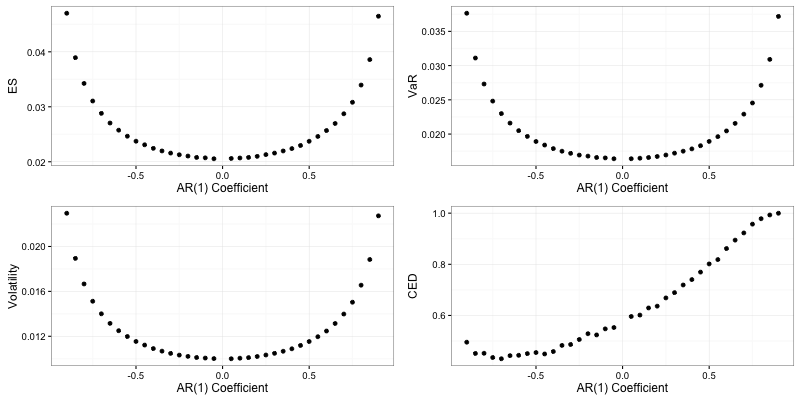
\includegraphics[width = 0.8\textwidth]{../figures/simulation/AR1_risk_measures}
\caption{AR(1): Relationship between auto-correlation coefficients and risk measures}
(Simulation path length: 1000, $\epsilon_t \sim N(0, 0.0001)$)
\label{fig:AR1_risk_measures}
\end{figure}

\begin{figure}[H]
\centering
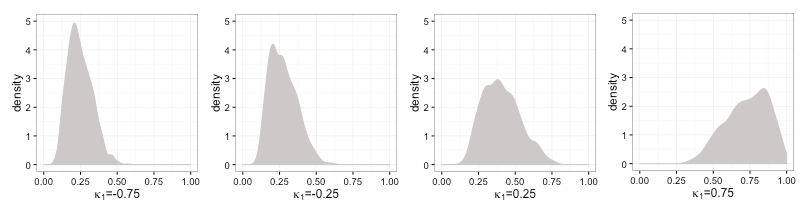
\includegraphics[width = 0.8\textwidth]{../figures/simulation/AR1_maxDrawdown_dist_re}
\caption{AR(1): Maximum drawdown distribution for various $\kappa_1$ values }
(Empirical distribution, path length = 1000, sample size = 1000, $\epsilon_t \sim N(0, 0.0001)$ )
\label{fig:AR1_maxDrawdown_dist}
\end{figure}

\subsection{GARCH model}
The previous several sections have already stated general ideas that how magnitude of risk measurements correlated with serial correlation and ARMA coefficients in AR(1), MA(1) and ARMA(1,1) models. However, the inspiring results should not encourage us ignore the complexity of the market: it always does not produce such regular time series. The occasional events shock the market and the returns always shows clustered variance. As has been analyzed in the Section \ref{garch}, a popular way to handle the complex variance in the return is using generalized autoregressive conditional heteroskedasticity (GARCH) model. In this section, ARMA time series are simulated with GARCH(1,1) noise term, to which we expect analysis the extent of effect that complex noise term having on the relationship between serial correlation and risk measurements.

Several universal assumptions around GARCH term in this section should be stated at this point. The GARCH model is on the basis of the Gaussian conditional distribution. Although in the empirical study with thirteen American indices it shows that a heavy tail conditional distributions, such as t-Student, are more likely to approximate the true market, Gaussian enable us to analyze more properties in the return without losing the generality. For GARCH(1,1), recall  that:
\[
\sigma^2_t = \omega + \alpha y_{t-1}^2 + \beta \sigma^2_{t-1}
\]The choose of potential parameters is on account of the study of the American financial indices. In summary, we choose $\omega \in \{10^{-7}, 10^{-8}\}$, $\alpha \in \{0.05, 0.08, 0.11, 0.14, 0.17, 0.20\}$, $\beta  \in \{0.1,0.2,\dots, 0.7\}$.

\subsubsection{AR(1)$\sim$GARCH(1,1)}
Started from the simpliest model AR(1)$\sim$GARCH(1,1), the simulation results provides us a general idea how risk measures changes with $\alpha$ and serial correlation, namely, $\kappa(1)$. Two questions are focused here 1) which parameter within $\omega$, $\alpha$ and $\beta$ are more responsible for the change in risk measurements? 2) Comparing the extent that the risk measurements changing with serial correlation or coefficients, does $\alpha$ and $\beta$ counts a lots?
\begin{figure}[H]
  \centering
  \begin{minipage}[b]{0.48\textwidth}
  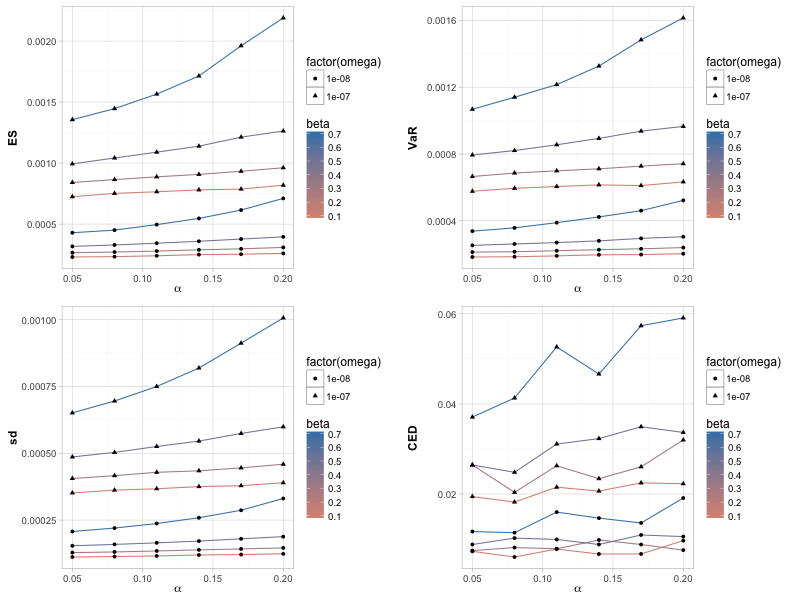
\includegraphics[width = 0.9\textwidth]{../figures/simulation_garch/garch_AR1_risk_measures_neg_alpha.png}
\caption{AR(1): Relationship between $\alpha$ parameter in the GARCH(1,1) and risk measures. The plots are produced under $\kappa_1 = -0.25$.}

\label{fig:garch_rm_alpha1}
  \end{minipage}
  \hfill
  \begin{minipage}[b]{0.48\textwidth}
   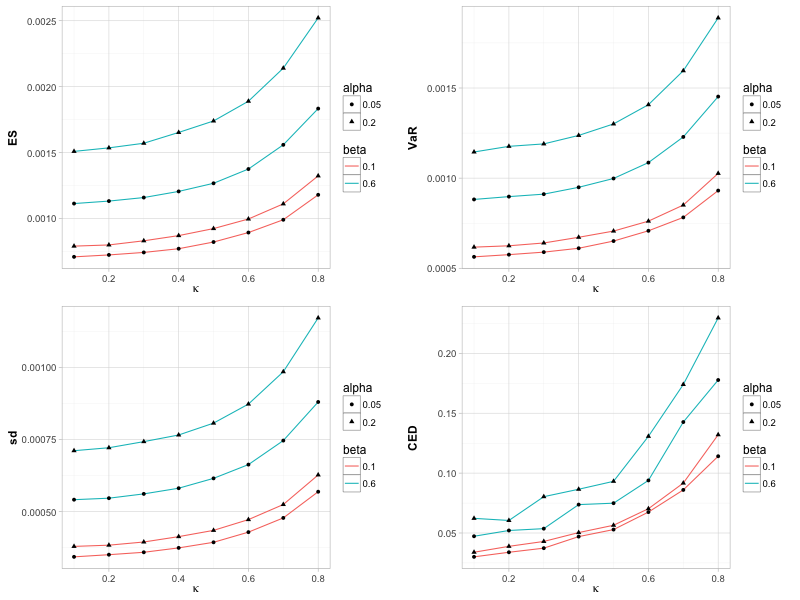
\includegraphics[width = 0.9\textwidth]{../figures/simulation_garch/garch_AR1_risk_measures_ar1}
\caption{AR(1): Relationship between serial correlation in the GARCH(1,1) and risk measures. $\kappa_1 \in \{0.1,0.2, \dots, 0.8 \}$}
%(Simulation path length: 1000, $\epsilon_t \sim 0.01T(df = 4)$)
\label{fig:garch_rm_coef1}
  \end{minipage}
\end{figure}

The Figure \ref{fig:garch_rm_alpha1} verifies our guess. The higher $\omega$, $\alpha$ or $\beta$ are all partial responsible for a highly risk measurements, in general. The eight lines within the plots are clearly separate into two groups, upper and lower. The higher four curves own a higher $\omega$, which indicates a general magnitude of variance. It is save to conclude that $\omega$ is dominant among parameters.

ES, VaR and Volatility are monotonically increasing with $alpha$. When the $\beta$ is relatively small, this relationship is almost linear, while when the $\beta$ is large, the relationship is more likely to be a higher order polynomial shape. In general, the CED has a similar trend with other risk measures, while it is less smooth. Especially, when the $\beta$ is low, $\alpha's$ effect is even more unclear. Indicating in the plot is the lowest three lines are twisting together. 

Figure \ref{fig:garch_rm_coef1} explores the how large $\omega$, $\alpha$ or $\beta$ affect the risk measurements comparing with changing in serial correlation. As proved, we only choose the positive coefficients to see the clear trend. With in $\alpha$ and $\beta$, the $\beta$ is dominant, especially in the first three plots, the 0.5 change in $beta$ is larger than 0.7 change in $\kappa$, fixed $\alpha$. A more exciting pattern shown in the CED plot. It shows that the complex variance, $\alpha$ or $\beta$ less affect CED, comparing the other risk measurements. In general, the curve in last plot is steeper, suggesting that CED is more sensitive to$\kappa$ in AR(1) $\sim$GARCH(1,1) model.

\subsubsection{ARMA(1,1) $\sim$GARCH(1,1)}
Similar to AR(1)$\sim$GARCH(1,1) model, we generalize it to ARMA(1,1)$\sim$GARCH(1,1), a more popular model in financial area.

In Figure \ref{fig:garch_ARMA11_risk_measures_3_alpha} where $\kappa_1 = 0.25$, $\theta_1 = -0.25$, the CED increases with the $\alpha$ and more sensitive when $\beta$ is high. Again, the $\omega$ is also the dominant factor compared with $\alpha$ and $\beta$.


\subsubsection{A short summary about GARCH}
This section is targeted in analyzing the impact of complex variance on the evaluation relationship of serial correlation($\kappa$ or $\rho$) and risk measures. It is more straightforward to see this effects through the simulation study other than tedious derivations. Through the analysis above, we have several conclusions as followed.

\begin{enumerate}
\item The larger value of $\omega$, $\alpha$ and $\beta$ are all partially responsible for a higher risk measurements, in general, given the ARMA model.
\item Among three parameters, the effect of $\omega$ dominates. As $\omega$ indicates the general change of variance of the model, which is a counterpart of $\sigma^2$ in the pure ARMA.
\item When the $\beta$ is small, the effect of $\alpha$ on risk measurements are weak. Especially for CED, it is insensitive to the change of $\alpha$. However, when the $\beta$ value is large, the ES, VaR and Volatility increase sharply with $\alpha$. For CED, it has a upward trend, but more indented than other risk measurements.
\item From the plots with $\kappa$ as axis, we found that in the time series with a GARCH variance, $\alpha$ and $\beta$ less affect CED comparing with other risk measurements.
\item Last but not least, we found that $\alpha$ value of the GARCH model does not change the shape of maximun drawdown distribution a lot compare with $\beta$ values. Therefore, in summary, for CED, the ranking magitude of effect from GARCH parameters are: $\alpha < \beta < \omega$
\end{enumerate}

\subsection{Findings}

In this section, we present findings summarized from the previous simulation study, and provide the corresponding theorial explainations. 

\textbf{1. CED distinguishes negative from positive autocorrelation}

For time series with positive autocorrelation, return is more likely to remain the same sign as the previous day. The likelihood increase as the serial correlation increase. As a consequence, returns tend to keep they current profit or loss status for a period. If the current status is loss, then unfortunately, the price of the asset may continuously go down, which results in a large CED. Conversely, time series with negative autocorrelation tend to reverse the sign in the previous day. If the the price of one assets goes down in one day, it is more likely that the price would bounce back in the next day, which results in alternating profit and loss status thus a smaller CED.

While CED captures the difference in serial correlation, other risk measures do not. VaR, ES and volatility are obtained from the empirical distribution of returns. If we shuffle the return sequence, we would get the same value for VaR, ES, and volatility.

Figure \ref{fig:Comparison_pos_neg_autocorrelation} shows the comparison of simulated returns and prices when serial correlation is 0.7 and -0.7. The maximum drawdown of simulated series is 22.76\% and 9.49\% separately. And two return series have the same VaR, ES and volatility.

\begin{figure}[H]
\centering
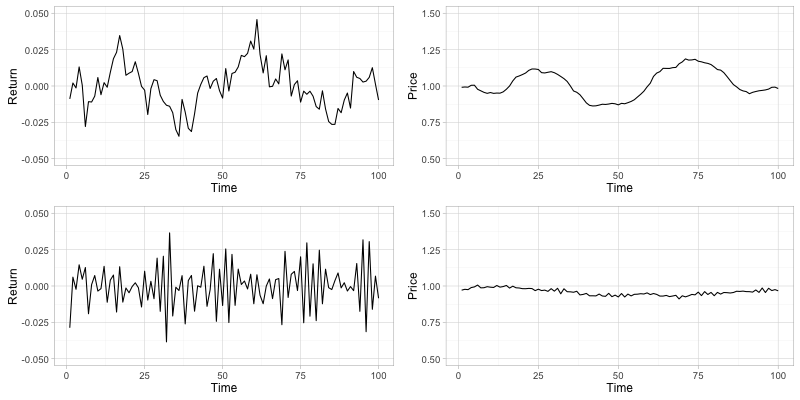
\includegraphics[width = 0.8\textwidth]{../figures/simulation/Comparison_pos_neg_autocorrelation}
\caption{Comparison of returns with positive and negative serial correlation}
(Simulation length: 100; upper panel: AR(1) with $\kappa=0.7$; lower panel: AR(1) with $\kappa=-0.7$, $\epsilon\sim N(0, 0.0001)$)
\label{fig:Comparison_pos_neg_autocorrelation}
\end{figure}

\textbf{2. Change standard deviation but fix everything in time series simulation would result in linear change of risk measures}

Simulation in Figure \ref{fig:change_std_simulation} for AR(1) model shows a linear relationship for all risk measures. We simulate the model $X_t = 0.3X_{t-1} + \epsilon_t$ and change the $\epsilon_t$ from 0.001 to 0.015.

\begin{figure}[H]
\centering
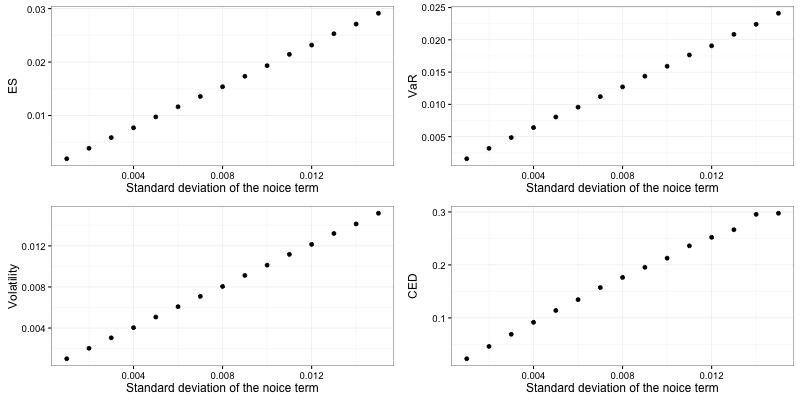
\includegraphics[width = 0.8\textwidth]{../figures/simulation/AR1_risk_measures_change_sd}
\caption{Comparison of returns with positive and negative serial correlation}
(Simulation length: 100; upper panel: AR(1) with $\kappa=0.7$; lower panel: AR(1) with $\kappa=-0.7$, $\epsilon\sim N(0, 0.0001)$)
\label{fig:change_std_simulation}
\end{figure}

Fixing everything but changing the standard deviation of the noise term would simply equals to multiplying the simulated time series model by a constant. For volatility, ES and VaR, it is obvious. For accumulated returns in a path, the return is approximately the sum of all returns for each day in this time period when the return is small (which is often the case):

\begin{equation}
R = \prod_{i=1}^n (1+r_i) - 1 \simeq \prod_{i=1}^n e^{r_i} - 1 = e^{\sum_{i=1}^n r_i} - 1 
 \simeq  \sum_{i=1}^n r_i
\end{equation}

All the returns in every subpath would be multiplied by approximately a constant. Thus, the domain of the maximum drawdown distribution and CED would also be scaled by the same number.

\section{Risk contribution}
Started from AR(1), present an example how risk contribution varied for different risk measurements, different weight and different ARMA parameters.\\

High light difference between CED and traditional risk measurements.\\

Short discuss how CED useful in capture the risk of financial assets on risk contribution aspect.


\clearpage

\newpage
\appendix
\section{Appendix A: Dataset} \label{App:AppendixA}
\subsection{Description}
\begin{table}[H]
\centering 
\begin{tabular}{ | r | p{7cm}  | p{4.5cm} | } 
 \hline 
Symbol & Name & Date range \\ \hline
AGG & iShares Core US Aggregate Bond & 2003-09-29 to 2015-12-31 \\
HYG & iShares iBoxx High Yield Corporate Bond & 2007-04-12 to 2015-12-31 \\
TIP & iShares TIPS Bond & 2003-12-08 to 2015-12-31 \\
BCOM & Bloomberg Commodity Index & 1991-01-03 to 2015-12-31 \\
G0O1 & 3-Month U.S. Treasury Bill Index & 1992-04-01 to 2015-12-31 \\
MXEA & MSCI Developed Markets Index & 1970-01-07 to 2015-12-31 \\
MXEF & MSCI Emerging Markets Index & 1988-01-01 to 2015-12-31 \\
RAY & Russell 3000 Index & 1979-01-02 to 2015-12-31 \\
RMZ & MSCI US REIT Index & 2005-06-20 to 2015-12-31 \\
SPX & S\&P 500 Index & 1950-01-04 to 2015-12-31 \\
USGG10YR & US Generic Govt 10 Year & 1962-01-03 to 2015-12-31 \\
 \hline
\end{tabular}
\caption{Normal VaR and ES under various levels}
\label{table:AssetDescription}
\end{table}


\subsection{Statistical summary}
annualized return, Sharpe Ratio, standard deviation, skewness, kurtosis [Empirical Page 8]

\subsection{Return}
Return across time and Return distribution [Empirical Page 8]

\subsection{Normal VaR and ES}

\begin{table}[H]
\centering 
\begin{tabular}{ | r || p{1cm} p{1cm} p{1cm} || p{1cm} p{1cm} p{1cm} | } 
 \hline
 & & VaR(\%) &&& ES(\%) & \\
Asset& 0.90 & 0.95 & 0.99 & 0.90 & 0.95 & 0.99 \\
  \hline \hline
AGG & 0.39 & 0.51 & 0.72 & 0.57 & 0.67 & 0.86\\ 
HYG & 1.06 & 1.36 & 1.94 & 1.50 & 1.76 & 2.26\\ 
TIP & 0.51 & 0.66 & 0.94 & 0.74 & 0.86 & 1.11\\ 
BCOM & 1.20 & 1.54 & 2.18 & 1.65 & 1.94 & 2.50\\ 
MXEA & 1.22 & 1.57 & 2.24 & 1.74 & 2.04 & 2.62\\ 
MXEF & 1.42 & 1.83 & 2.61 & 2.03 & 2.38 & 3.06\\ 
RAY & 1.36 & 1.75 & 2.49 & 1.95 & 2.29 & 2.94\\ 
RMZ & 2.92 & 3.75 & 5.32 & 4.08 & 4.79 & 6.18\\ 
SPX & 1.21 & 1.57 & 2.22 & 1.73 & 2.03 & 2.61\\ 
USGG10YR & 1.62 & 2.08 & 2.95 & 2.23 & 2.62 & 3.39\\
 \hline
\end{tabular}
\caption{Normal VaR and ES under various levels}
\label{table:VaRESNormal}
\end{table}



\section{Appendix B: Rolling risk diagnostics} \label{App:AppendixB}

\begin{figure}[H]
\centering
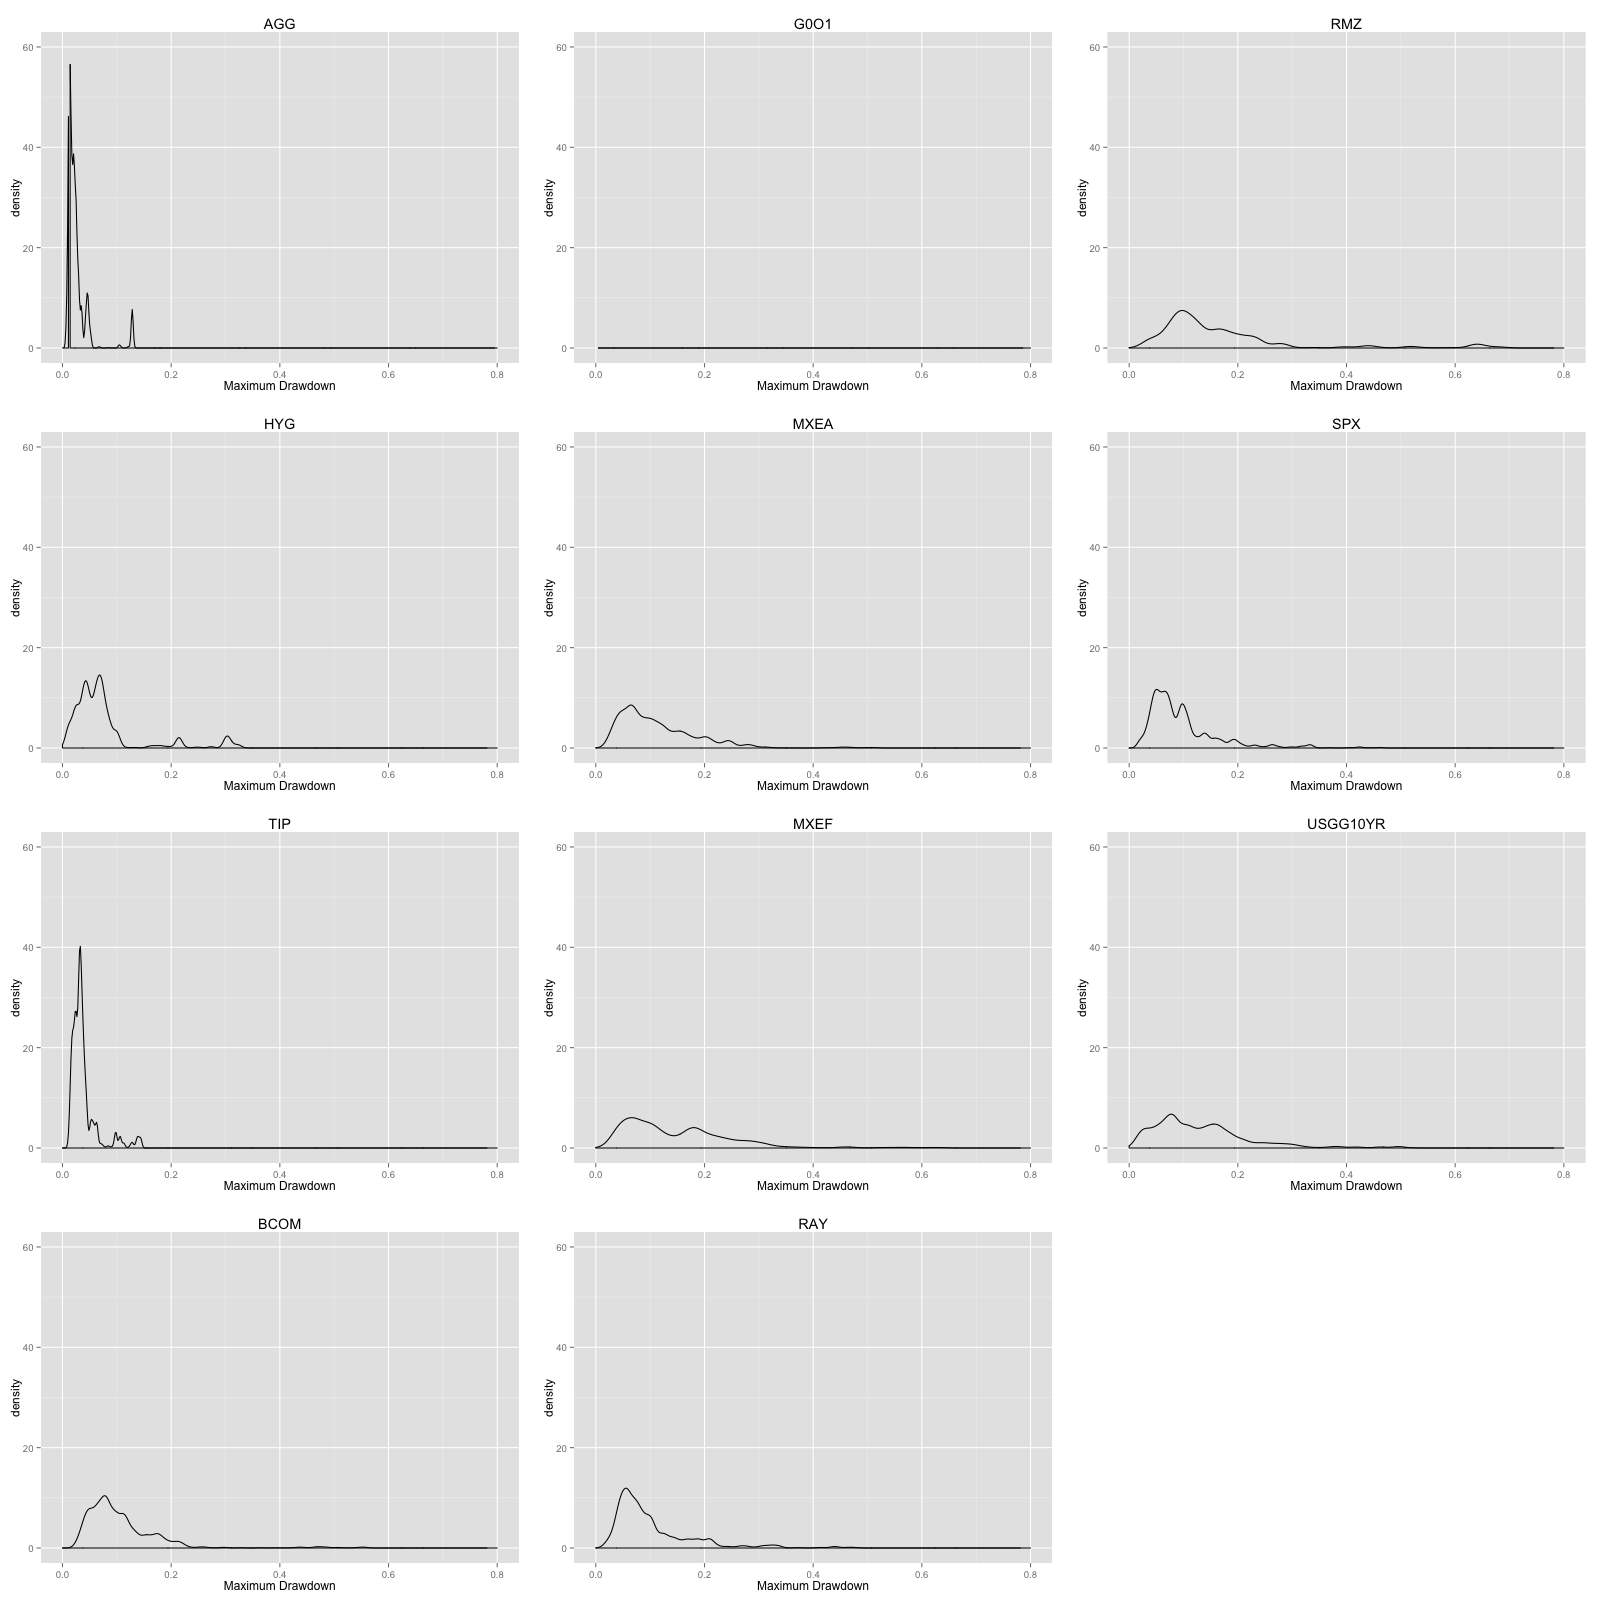
\includegraphics[width=15cm]{../results/maxdd_dist_mon6}
\caption{Empirical distribution of maximum drawdown under 6 month rolling window} 
\label{fig: dist_mdd}
\end{figure}

\begin{table}
\caption{Correlation between CED (confidence level = 0.9) and other risk measures}
\centering 
\begin{tabular}{| p{2cm}||p{2cm}|p{2cm}|p{2cm}|} 
\hline
Measures & Volatility & VaR & ES\\
  \hline
AGG & 0.94 & 0.89 & 0.95\\ 
HYG & 0.98 & 0.97 & 0.97\\ 
TIP & 0.77 & 0.85 & 0.85\\ 
BCOM & 0.84 & 0.89 & 0.89\\ 
MXEA & 0.84 & 0.83 & 0.86\\ 
MXEF & 0.91 & 0.91 & 0.93\\ 
RAY & 0.92 & 0.85 & 0.92\\ 
RMZ & 0.96 & 0.96 & 0.97\\ 
SPX & 0.84 & 0.81 & 0.84\\ 
USGG10YR & 0.91 & 0.93 & 0.95\\
\hline
\end{tabular}
\label{table:corrRiskMeasureCED}
\end{table}

\begin{table}
\caption{Summary statistics of two regimes for various assets} 
\centering 
\begin{tabular}{ | c || rr | rr | rr | } 
 \hline
& \multicolumn{2}{c|}{Volatility} & \multicolumn{2}{c|}{Skewness} & \multicolumn{2}{c|}{Kurtosis} \\
Asset & Regime 1 & Regime 2 & Regime 1 & Regime 2 & Regime 1 & Regime 2 \\
  \hline \hline
AGG & 0.141 & 0.036 & -1.59 &  0.01 & 17.15 &  0.60\\ 
HYG & 0.265 & 0.055 &  0.60 &  0.00 &  8.76 &  0.83\\ 
TIP & 0.113 & 0.049 &  0.18 & -0.06 &  2.50 &  0.16\\ 
BCOM & 0.205 & 0.096 & -0.25 & -0.04 &  1.92 &  0.28\\ 
MXEA & 0.253 & 0.101 & -0.14 & -0.02 &  4.26 &  0.25\\ 
MXEF & 0.303 & 0.119 & -0.08 & -0.06 &  2.39 &  0.38\\ 
RAY & 0.307 & 0.114 & -0.39 & -0.06 &  6.43 &  0.55\\ 
RMZ & 0.661 & 0.159 &  0.29 & -0.15 &  2.92 &  0.79\\ 
SPX & 0.260 & 0.099 & -0.43 & -0.02 &  9.11 &  0.56\\ 
USGG10YR & 0.314 & 0.098 &  0.09 & -0.05 &  2.67 &  1.17 \\
 \hline
\end{tabular}
\label{table:statSumRegime}
\end{table}

\section{Appendix C: Simulations specifics} \label{App:AppendixC}
\subsubsection{Noise term with normal distribution}

We use some simple assumptions and parameters for simulation with normal distribution as follows:

\begin{enumerate}
\item Noise terms in the time series model follow Normal distribution with standard deviation of 0.01: $\epsilon \sim N(0, 0.0001)$.
\item Risk measures including volatility, VaR, ES and maximum drawdown are calculated based on simulated time series with path length 1000. The calculation of maximum drawdown is replicated 1000 times in order to obtain the maximum drawdown distribution and its tail mean (CED).
\item All time series parameters in this section range from -0.9 to 0.9. For time series with multiple parameters such as AR(2), ARMA(1, 1), the parameters are cartesian product of arithmetic progressions range from -0.9 to 0.9. Note that to take the stationary of AR and ARMA models into consideration (all moving averages are stationary, but the AR and ARMA model have to meet certain criteria to be stationary), not all parameters in the cartesian product are used in the simulation.
\end{enumerate}


\section{Appendix D: Empirical Study Results} \label{App:AppendixD}
\begin{figure}[H]
  \centering
  \begin{minipage}[b]{0.48\textwidth}
    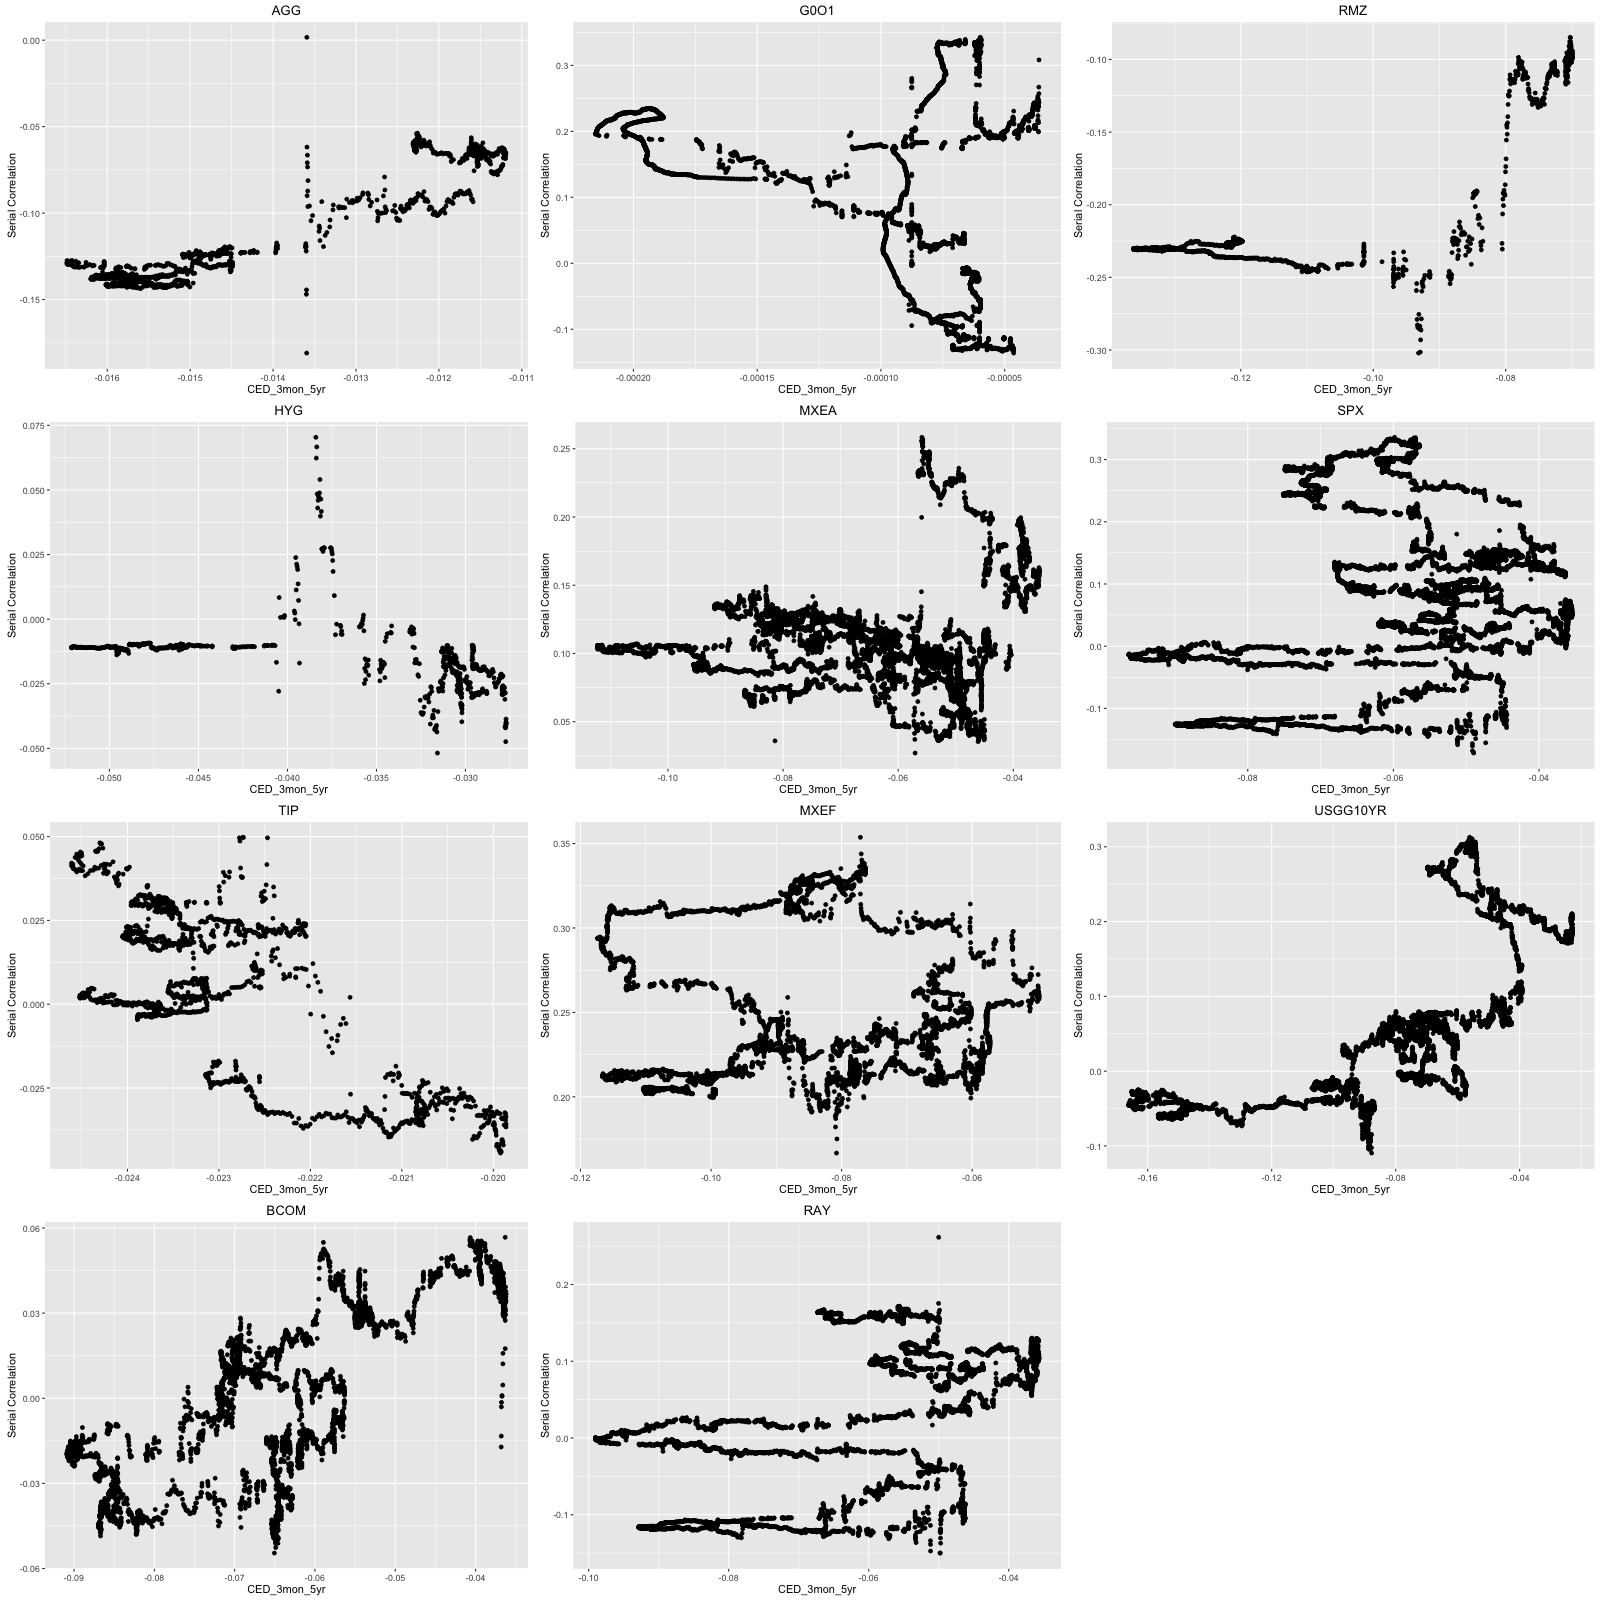
\includegraphics[width=\textwidth]{../results/SerCol-CED5yr3monAR1}
    \caption{First-order serial correlation calculated using AR(1) model versus CED}
    \label{fig:SerCol-CED5yr3monAR1}
  \end{minipage}
  \hfill
  \begin{minipage}[b]{0.48\textwidth}
    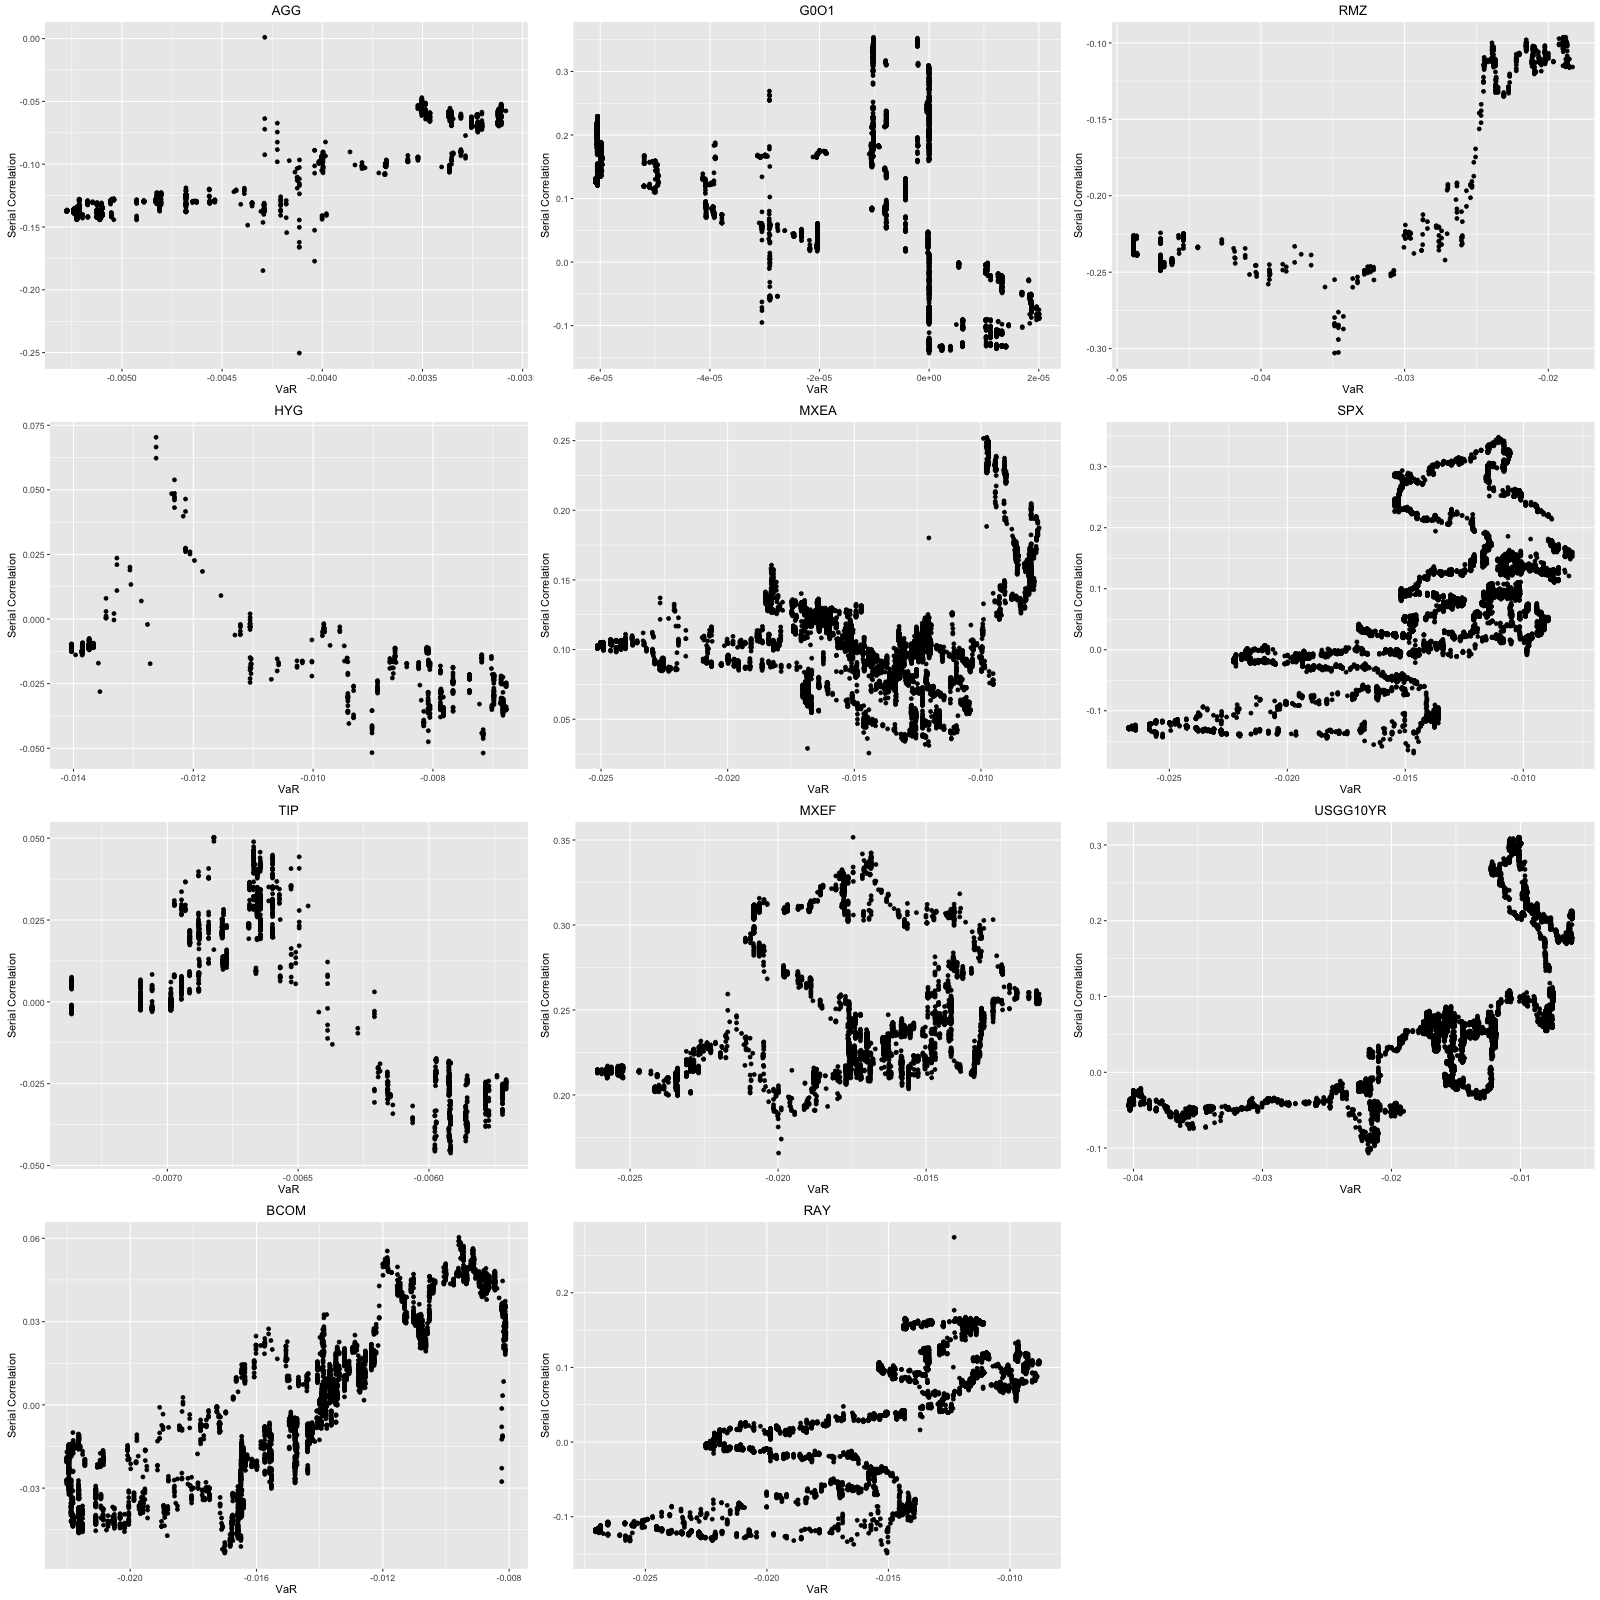
\includegraphics[width=\textwidth]{../results/SerCol-VaR5yrAR1}
    \caption{First-order serial correlation calculated using AR(1) model versus VaR}
    \label{fig:SerCol-VaR5yrAR1}
  \end{minipage}
\end{figure}

\subparagraph{Model Selection Criteria}




\newpage

\bibliographystyle{unsrt}
\bibliography{analysis}






\clearpage


===========Overall risk measures for various assets============

(Use unannualized VaR, ES and volatility in order to compare)

VaR, ES: Empirical method \& normal method, VaR and ES is being overestimated at a lower confidence level and being underestimated at a higher confidence level. [Empirical, Page 49]

Volatility: [Empirical, Page 8]

Overall CED: how they are different under different confidentce interval and rolling windows [Empirical, Page 10]

Relationship between risk measures: assets with larger VaR, ES and volatility also have larger CED, give the correlation values, Do they give the same order from lowest risk asset to highest?[Empirical, Page 10]

Asset with largest and smallest risk for each risk measures: relate this with intuitive sence and the component of asset class. [Empirical, Page 9]

Relative values of different assets for different risk measures: Is there a risk measure distinguish assets from each other most? [To be added]


===========Time-varying risk diagnostics=============

Empirical distribution of maximum drawdown is sensitive to the time length of measurement. [Empirical, Page 11, Figure 1]

Large windows not desirable, why? [Empirical, Page 11, 13, Figure 1; Presentation2 Page3]

Correlation between risk measures over time [Empirical, Table 4, 5, Figure 2, 27]

CED plot

Risk measures, when biggest? related to real world events. [To be extended]

=============== regime switching model ======

Introduction [Summary Page 13]

Summary of regime switching model for different assets [Summary Page 13][To be add: modeled variance]

Why can not see strong correlation between serial correlation and CED? Relate this to the simulation study: when both volatility and seiral correlation are different, volatility usually dominant the influence for CED. [To be added]

Rolling risk measure (RMZ as example): Correlation between seial correlation and risk measure for two regions [Empirical Page 15]

================ simulation summary =========

AR, MA and ARMA model with normal dist and t dist, fat tail distribution would result in more randomness when calculating CED and other risk measures[Simulation Page 2 - 21]

Garch model fitting: how different coefficients influence the risk measure values? [Simulation Page 32]

Simulation with standard error adjusted [Simulation Page 21]

CED distinguishes negative from positive autocorrelation[Simulation Page 21]

Change standard deviation but fix everything in time series simulation would result in linear change of risk measures[Simulation Page 22]

The influence of volatility dominant in the risk measure calculation, relate this to empirical data, why usually we can not discover patterns? [To be added] 

==============================================

Which model gives the best fit (statistically)? Which assets have strongest serial correlation? The point here is to to understand the autocorrelation behavior of vaious asset classes, so you should once again interpret your results and parameters.

relationship of the time series of the serial correlation parameters (e.g. $\kappa$ in the AR(1) model) with the time series of the various risk diagnostics. Is serial correlation strongly related to volatility, ES, VaR and CED? Is it more strongly correlated to one risk measure than another?



Part I: Empirical analysis

1. Understand the different risk characteristics (particularly drawdown) of different asset classes.

2. Comparing the insights gained by looking at the maximum drawdown distribution in addition to the returns distribution.

3. Find the empirical relationship between serial correlation and risk.


Part II: Simulations

1. Comparison of risk measures of various simulated models.

2. Comparison of the returns and maximum drawdown distribution for various simulated models. (parallel to point 2 above)

3. Relationship between serial correlation and risk based on simulated models. (parallel to point 3 above)


The answer is that simulation and empirical analysis are two elements that play a complementary role in our understanding of the financial world, and specifically of drawdown risk: empirical analyses roughly guide us in understanding what are economically reasonable assumptions. Simulations help us estimate models from data generated by a known process. These simulated models are often used in practice for the purpose of forecasting and are tested out-of-sample for accuracy on empirical data. (Note however that forecasting will not be part of your project.)


Our hypothesis for this next part is that higher serial correlation would result in higher drawdown risk concentrations (compared with risk concentrations along the other risk measures). Here is an outline of what you can do:

1. Simulate the returns to two assets E (representing equity) and B (representing Bonds). For each model you simulate (AR, MA, GARCH, combination models, etc), you can use the parameters obtained by fitting to the real time series of equity and bonds (which you already have). Moreover, if your error term is Gaussian, you could use the real volatility of the underlying assets for the simulation.

2. For each model you simulate, construct 50/50, 60/40, and 70/30 portfolios.

3. For each model and portfolio, calculate the overall fractional risk contributions to volatility, ES, and CED along assets E and B.



\end{document}